\NeedsTeXFormat{LaTeX2e}
\documentclass[a4paper,12pt]{monografia}
\usepackage{hyperref}
\hypersetup{colorlinks, debug=false, linkcolor=black, citecolor=black, urlcolor=black, bookmarksopen=true}
\usepackage[portuguese, colorinlistoftodos, textsize=tiny]{todonotes}
\usepackage{amsmath,amsthm,amsfonts,amssymb}
\usepackage[mathcal]{eucal}
\usepackage{latexsym}
\usepackage[portuguese]{babel}  
\usepackage[utf8]{inputenc}
\usepackage{setspace}
%\usepackage{natbib}
\usepackage{bm}
\usepackage[portuguese,algoruled,longend, linesnumbered]{algorithm2e}
\usepackage{listings}
\usepackage{graphicx}
\usepackage[alf,bibjustif]{abntex2cite}
\newcounter{todocounter}
\newcommand{\comment}[2][]
{\stepcounter{todocounter}\todo[caption={\thetodocounter: #2}, #1] 
{\begin{spacing}{1}\thetodocounter: #2\end{spacing}}}
\reversemarginpar
\setlength{\marginparwidth}{2.5cm}
\lstloadlanguages{C}
\theoremstyle{plain}
\newtheorem{theorem}{Teorema}[section]
\newtheorem{axiom}{Axioma}[section]
\newtheorem{corollary}{Corol\'ario}[section]
\newtheorem{lemma}{Lema}[section]
\newtheorem{proposition}{Proposi\c{c}\~ao}[section]
\theoremstyle{definition}
\newtheorem{definition}{Defini\c{c}\~ao}[section]
\newtheorem{example}{Exemplo}[section]
\theoremstyle{remark}
\newtheorem{remark}{Observa\c{c}\~ao}[section]
\newcommand{\R}{\mathbb{R}}
\newcommand{\N}{\mathbb{N}}
\newcommand{\Z}{\mathbb{Z}}
\newcommand{\Q}{\mathbb{Q}}
\newcommand{\K}{\mathbb{K}}
\newcommand{\I}{\mathbb{I}}
\newcommand{\id}{\mathbf{1}}
\newcommand{\U}{\mathcal{U}}
\newcommand{\V}{{\cal V}}
\def\ind{\hbox{ ind }}

\usepackage{color}
\newcommand{\abv}[1]{\textcolor{red}{\bf [Alex]: #1}}

\hyphenation{Con-si-de-ra-mos}
\hyphenation{me-lhor}
\hyphenation{res-pos-ta}
\hyphenation{re-qui-si-tos}

\begin{document}
\titulo{Loteria Descentralizada em Blockchain EOSIO}
%\subtitulo{$<<$Subt\'itulo - opcional$>>$}
\autor{Ricardo de Barros Marli\`ere} \nome{Ricardo} \ultimonome{Marli\`{e}re}
\bacharelado
\curso{Sistemas de Informa\c{c}\~ao} 
\dia{29} \mes{Dezembro} \ano{2018}
\cidade{Juiz de Fora}
\instituicao{Universidade Federal de Juiz de Fora} \sigla{UFJF}
\unidadeacademica{Intituto de Ci\^encias Exatas}
\departamento{Departamento de Ci\^encia da Computa\c{c}\~ao}
\orientador{Alex Borges Vieira}
\ttorientador{Doutor em Ci\^encia da Computa\c{c}\~ao}
%\coorientador{$<<$Nome do Co-orientador$>>$}
%\ttcoorientador{$<<$T\'itulo do Co-orientador$>>$} 
\examinadorum{Helo\'isa Pinna Bernardo}
\ttexaminadorum{Doutora em Contabilidade e Controladoria}
\examinadordois{M\'ario Ant\^onio Ribeiro Dantas}
\ttexaminadordois{Doutor em Ci\^encia da Computa\c{c}\~ao}
%\examinadortres{Nome do Examinador 3}
%\ttexaminadortres{T\'itulo do Examinador 3}
%\examinadorquatro{Nome do Examinador 4}
%\ttexaminadorquatro{T\'itulo do Examinador 4}
%\CDU{536.21} \areas{1.Análise Matemática  2. Topologia.}
%\npaginas{xx}  % total de páginas do trabalho
\inserirlogo  
\maketitle







%\begin{dedicatoria}
%\end{dedicatoria}

\resumo{Resumo}
Em 2008, um pesquisador an\^onimo publicou sua mais nova inven\c{c}\~ao: o Bitcoin, protocolo ponto a ponto de dinheiro eletr\^onico descentralizado que est\'a rapidamente causando mudan\c{c}as significativas no setor financeiro.
Menos de 10 anos depois, sua tra\c{c}\~ao continua forte atraindo cada vez mais investidores e especuladores, inaugurando uma nova sub\'area na Ci\^encia da Computa\c{c}\~ao que \'e o estudo das \textit{blockchains}.
Numerosos s\~{a}o os debates acerca da escalabilidade do sistema proposto por \citeonline{bitcoin} e, neste sentido, o foco deste trabalho \'e explorar de forma pr\'atica uma nova arquitetura escal\'{a}vel proposta por \citeonline{eos}, chamada EOSIO.

\noindent \\ \textbf{Palavras-chave:} Bitcoin, criptomoeda, descentraliza\c{c}\~ao, \textit{blockchain}, EOSIO

\resumo{Abstract}
In 2008, an anonymous researcher published his newest invention: the Bitcoin, a peer to peer decentralized protocol of electronic cash that is quickly and significantly disrupting the finantial sector.
Less than 10 years later, its traction keep steadily growing and attracting more and more investors and speculators, inaugurating a new subarea of Computer Science which is the study of blockchains.
There are great and extensive discussions about the scalability of the system proposed by \citeonline{bitcoin} and, in that sense, the goal of this work is to explore a new scalable architecture called EOSIO, proposed by \citeonline{eos}, in a practical manner.

\noindent \\ \textbf{Keywords:} Bitcoin, \textit{cryptocurrency}, \textit{decentralization}, \textit{blockchain}, EOSIO

%\agradecimento{Agradecimentos} \indent\indent 
%A todos os meus parentes, pelo encorajamento e apoio.

\newpage

\begin{epigrafe}
``The joy of life consists in the exercise of one’s energies, continual growth, constant change, the enjoyment of every new experience. To stop means simply to die. The eternal mistake of mankind is to set up an attainable ideal''.\\
\hfill Aleister Crowley
\end{epigrafe}

\tableofcontents
\thispagestyle{empty}
\listoffigures
\thispagestyle{empty}
%\listoftables
%\thispagestyle{empty}

\chapter*{Lista de Abrevia\c{c}\~oes} \addcontentsline{toc}{chapter}{Lista de Abrevia\c{c}\~oes}
\doublespacing  \begin{tabular}{l l}
ABI  & Application Binary Interface\\
API  & Application Programming Interface\\
BIP  & Bitcoin Improvement Proposal\\
BTC  & Bitcoin\\
BP   & Block Producer\\
CAPTCHA & Completely Automated Public Turing test\\
    & to tell Computers and Humans Apart\\
CDT  & Contract Development Toolkit\\
CLI  & Command Line Interface\\
DAC  & Decentralized Autonomous Corporation\\
DAO  & Decentralized Autonomous Organization\\
Dapp & Decentralized Application\\
DPoS & Delegated Proof of Stake\\
ECAF & EOS Core Arbitration Forum\\
ETC  & Ethereum Classic\\
ETH  & Ethereum\\
EVM  & Ethereum Virtual Machine\\
JSON & JavaScript Object Notation\\
LCG  & Linear Congruential Generator\\
PRNG & Pseudorandom Number Generator\\
PoS  & Proof of Stake\\
PoW  & Proof of Work\\
RPC  & Remote Procedure Call\\
SDK  & Software Development Kit\\
UTXO & Unspent Transaction Output\\
\end{tabular}  \thispagestyle{empty}

\pagestyle{ruledheader}

\chapter{Introdu\c{c}\~ao}

A crescente demanda por criptomoedas por um p\'ublico cada vez mais abrangente \'e demonstrada atrav\'es do aumento significativo da capitaliza\c{c}\~ao do mercado ao longo dos \'ultimos anos.
Ao final de 2017, estima-se que o valor de mercado conjunto de todas as criptomoedas fosse superior \`a 800 bilh\~oes de d\'olares estadunidenses, sendo que mais de 45\% correspondiam apenas ao mercado de bitcoins em si\footnote{Dispon\'ivel em: \url{https://coinmarketcap.com/} (acesso em 17-11-2018)}.
Isto representa uma diferen\c{c}a muito acentuada para com o ano de 2016, onde o montante n\~{a}o excedeu muito al\'{e}m de 16 bilh\~{o}es.

Tal demanda fica justificada pelo fato da nova tecnologia inerente a estas moedas, chamada \textit{blockchain} (cadeia de blocos, em portugu\^{e}s), possibilitar transa\c{c}\~{o}es seguras de valor de forma direta entre as pessoas, sem uma institui\c{c}\~{a}o financeira como intermedi\'{a}ria.
Em momentos de crises econ\^{o}micas generalizadas, \'{e} pr\'{a}tica comum recorrer a metais preciosos para estabelecer o que \'{e} conhecido como reserva de valor e uma nova alternativa surge para tal com o advento das criptomoedas.
Prova disto \'{e} o aumento da procura por bitcoins em pa\'{i}ses afetados por grave infla\c{c}\~{a}o monet\'{a}ria como Venezuela e Zimbábue, o que resulta numa cota\c{c}\~{a}o interna muito superior ao restante dos mercados do mundo.

Por outro lado, por se tratar de um protocolo de rede ponto a ponto, criptomoedas podem ser utilizadas com motiva\c{c}\~{o}es eticamente duvidosas.
Ao contr\'{a}rio do sistema banc\'{a}rio, onde cada conta \'{e} sempre vinculada \`{a} identidade de algu\'{e}m, um endere\c{c}o sob controle de um n\'{o} da rede nem sempre pode ter sua pessoa rastreada.
Ao aliar o novo dinheiro eletr\^{o}nico que possui alto grau de anonimidade com um outro protocolo chamado Tor que obfusca o roteamento de pacotes para dificultar seu rastreio, Ross Ulbricht fundou em Fevereiro de 2011 uma das primeiras comunidades onde o Bitcoin foi adotado. O mercado negro chamado Silk Road, onde criminosos negociavam artigos il\'{i}citos usando a moeda, foi em parte grande respons\'{a}vel pela populariza\c{c}\~{a}o do tema e teve suas opera\c{c}\~{o}es completamente desativadas pelo FBI apenas em Outubro de 2013, com seu fundador condenado a cumprir pena vital\'{i}cia em regime fechado.

Tendo estabelecido o marco inicial em 2008 pela inven\c{c}\~{a}o da \textit{blockchain}, o \textit{cypherpunk} \cite{cypherpunk} Satoshi Nakamoto foi tamb\'{e}m respons\'{a}vel pela primeira implementa\c{c}\~{a}o do protocolo e permaneceu ativo como desenvolvedor at\'{e} 2010.
Desde ent\~{a}o, muitas evolu\c{c}\~{o}es v\^{e}m tomando forma tanto no contexto do pr\'{o}prio Bitcoin quanto em outros protocolos.
Os primeiros projetos de \textit{blockchains} independentes do Bitcoin que buscavam inovar e refinar o conceito datam de 2012 mas ainda h\'{a} muito o que ser explorado haja vista que s\~{a}o escassas as evid\^{e}ncias de casos de uso atualmente implementados que possuam alguma not\'{a}vel ado\c{c}\~{a}o pelo p\'{u}blico em geral que n\~{a}o seja uma simples moeda. 

Como \'{e} de conhecimento comum, a maior de todas as empresas que oferecem servi\c{c}os de transporte privado n\~{a}o possui frota alguma; de maneira semelhante, a empresa dona das m\'{i}dias da maior rede social do mundo n\~{a}o produz conte\'{u}do; o maior varejista n\~{a}o possui estoque; o maior provedor de acomoda\c{c}\~{o}es n\~{a}o possui im\'{o}veis.
A ado\c{c}\~{a}o em massa \'{e} um grande indicativo do sucesso de uma aplica\c{c}\~{a}o e os gigantes corporativos do setor da tecnologia demonstram que existe demanda para diversos casos de uso onde o valor \'{e} derivado diretamente da comunidade.
Com\'{e}rcio virtual, redes sociais, cassinos, cart\'{o}rios, elei\c{c}\~{o}es, cadeias de cust\'{o}dia, cadeias produtivas como por exemplo no rastreio e certifica\c{c}\~{a}o da origem de madeira ou diamantes, casas de c\^{a}mbio e bolsas (ou \textit{exchanges}, no ingl\^{e}s) e muitas outras aplica\c{c}\~{o}es podem ser modeladas como casos de uso descentralizados e passam a representar uma grave afronta aos modelos tradicionais por serem mais ou t\~{a}o seguros quanto, transparentes, aut\^{o}matos e potencialmente menos custosos.

\section{Problema}
O problema resolvido pelas \textit{blockchains} \'{e} a remo\c{c}\~{a}o de intermedi\'{a}rios em transa\c{c}\~{o}es de valor.
Indo al\'{e}m do Bitcoin e institui\c{c}\~{o}es financeiras, podem ser modelados muitos outros casos de uso amplamente adotados na atualidade atrav\'{e}s da cria\c{c}\~{a}o de contrapartes descentralizadas.
Para o \^{a}mbito deste trabalho, \'{e} proposta uma \textit{dapp} de loteria.

\section{Justificativa}
Utiliza-se o novo paradigma de neg\'{o}cio possibilitado pelo conceito da \textit{blockchain} para remover o intermedi\'{a}rio no contexto desta aplica\c{c}\~{a}o, pois a falta de transpar\^encia compromete a verifica\c{c}\~ao da satisfatoriedade estat\'istica de diversos jogos.

\section{Objetivo}
O sucesso de determinada tecnologia ou aplica\c{c}\~{a}o pode ser intuitivamente relacionado com o tamanho de sua base de usu\'{a}rios.
Apesar da \textit{blockchain} ser uma inven\c{c}\~{a}o recente, fato \'{e} que sua ado\c{c}\~{a}o \'{e} cada vez maior e a tend\^{e}ncia \'{e} permanecer em crescimento desde que mais casos de uso sejam implementados de forma descentralizada.
Para tanto, o objetivo da plataforma proposta neste trabalho \'{e} a cria\c{c}\~{a}o de uma comunidade de jogadores visando o aumento da base de usu\'{a}rios de solu\c{c}\~{o}es descentralizadas como um todo.

\section{Metodologia}
Para tornar vi\'{a}vel o desenvolvimento deste trabalho, um mapeamento da literatura \'{e} necess\'{a}rio para estabelecer a base te\'{o}rica e devida contextualiza\c{c}\~{a}o do tema via exemplos.
Segue-se ent\~{a}o para a especifica\c{c}\~{a}o dos requisitos da aplica\c{c}\~{a}o que s\~{a}o por sua vez utilizados para modelar a arquitetura da mesma.

\chapter{Fundamenta\c{c}\~ao Te\'orica}

O objetivo do presente cap\'itulo \'e apresentar um hist\'orico e panorama geral das principais tecnologias presentes nas criptomoedas.
Na se\c{c}\~{a}o 2.1, aborda-se o protocolo pioneiro de dinheiro eletr\^{o}nico Bitcoin.
Na se\c{c}\~{a}o 2.2 o inovador Ethereum \'e visto em detalhes e por \'{u}ltimo, na se\c{c}\~{a}o 2.3, \'e feita uma an\'alise das possibilidades apresentadas pelo projeto EOSIO.

\section{Bitcoin}

Em 2008, um pesquisador conhecido apenas pelo pseud\^onimo Satoshi Nakamoto publicou um artigo simples de apenas oito p\'aginas em que apresenta um sistema ponto a ponto de dinheiro eletr\^onico que possui implica\c{c}\~oes sociais e econ\^omicas ainda a serem apreciadas em sua plenitude.
O Bitcoin torna poss\'{i}vel a transfer\^{e}ncia direta de valor entre dois pontos ao redor do mundo de forma segura, r\'{a}pida e barata.
Na pr\'{a}tica, o que ocorre \'{e} a remo\c{c}\~{a}o do atravessador (como, por exemplo, o pr\'{o}prio banco no contexto de transa\c{c}\~{o}es banc\'{a}rias), devido ao fato de ser uma rede descentralizada \cite{bitcoin}.
Respostas diversas s\~ao extra\'idas a depender de quem seja perguntado: Bitcoin poderia ser considerado, ao mesmo tempo, dinheiro program\'avel, uma nova classe de ativos, uma moeda, uma rede de computadores e uma commodity.

Note que, apesar de ser pioneiro na efetiva resolu\c{c}\~{a}o deste problema vinculado \`{a} moedas centralizadas, o Bitcoin n\~{a}o foi a primeira tentativa.
De fato, a primeira proposta de cria\c{c}\~ao de dinheiro eletr\^{o}nico, eCash \cite{ecash}, requeria dos usu\'arios que depositassem confian\c{c}a numa autoridade central, muito similar ao sistema banc\'ario.
Isso s\'o foi resolvido meio quarto de s\'eculo mais tarde por Satoshi Nakamoto ao criar um protocolo que tomou emprestado conceitos importantes oriundos de: Pretty Good Privacy \cite{pgp}, b-money \cite{b-money}, Proof of Work (PoW) \cite{pow}, Hashcash \cite{hashcash}, BitTorrent \cite{bittorrent}, Reusable Proofs of Work \cite{rpow}, Bit Gold \cite{bitgold}.

Parte-se da ideia de que, desde que dinheiro nada mais \'e que um sistema cont\'abil, o livro raz\~ao (\textit{ledger}) deve ser fielmente distribu\'ido a todos os pares membros da rede.
Por\'em, ao contr\'ario de um sistema centralizado em que o banco detecta fraudes em que se tenta gastar mais dinheiro do que se tem dispon\'ivel (no ingl\^es, \textit{double-spending}), o mesmo n\~ao \'e t\~ao simples num sistema distribu\'ido.
Afinal, c\'opias digitais s\~ao triviais de serem feitas e \'e necessario um mecanismo de
armazenamento em que a situa\c{c}\~ao seja improv\'avel.
Este problema foi resolvido com o Bitcoin.
Para tal, \citeonline{bitcoin} prop\^os "uma rede ponto-a-ponto que usa PoW para registrar um hist\'orico p\'ublico de transa\c{c}\~oes que rapidamente se torna computacionalmente impratic\'avel para um atacante o alterar se n\'os honestos controlarem a maior parte do poder de CPU".

Dentre as principais caracter\'isticas do protocolo, pode-se citar em destaque as tr\^es maiores que evidenciam a verdadeira quebra de paradigmas trazida \`a tona pelo Bitcoin:

\begin{enumerate}
\item Existe um limite imposto pelo \textit{software} de forma que o total de bitcoins em circula\c{c}\~ao jamais ser\'a superior a 21 milh\~oes, o que a torna deflacion\'aria partindo da hip\'otese de demanda crescente.
\item A impress\~ao de novas moedas n\~ao depende da autoridade de um Banco Central, o que a torna livre de quaisquer fronteiras\footnote{Entretanto, derivativos (contratos futuros) servem como ferramenta para autoridades e grandes institui\c{c}\~oes financeiras controlarem o pre\c{c}o da moeda, tal como \'e feito nos mercados de metais preciosos e outras \textit{commodities} \cite{nakedshort}.}.
\item Pela primeira vez na hist\'oria da humanidade, pessoas comuns n\~ao precisam recorrer a bancos para armazenamento e transfer\^{e}ncia seguras de valor\footnote{Chaves privadas ocupam o mesmo espa\c{c}o em disco independentemente da quantidade dispon\'{i}vel de bitcoins numa determinada carteira \cite{bitcoin}.}.
\end{enumerate}

As subse\c{c}\~{o}es a seguir visam elucidar os componentes e conceitos mais importantes do protocolo para que o mesmo possa ser mais facilmente entendido.
O mais importante \'{e} a transa\c{c}\~{a}o criptograficamente v\'{a}lida de moedas e ser\'{a} visto na subse\c{c}\~{a}o 2.1.1.
Tais transa\c{c}\~{o}es devem ser agrupadas em blocos e enumeradas de acordo com o \textit{timestamp} em que foram geradas, sendo os detalhes discutidos na subse\c{c}\~{a}o 2.1.2. Por \'{u}ltimo, a subse\c{c}\~{a}o 2.1.3 explica o mecanismo que incentiva os n\'{o}s da rede a permanecerem honestos.

\subsection{Transa\c{c}\~ao}

Uma transa\c{c}\~ao nada mais \'e que o envio de moedas de um endere\c{c}o a outro, anunciada publicamente  na rede.
\citeonline{bitcoin} definiu uma moeda eletr\^onica como uma cadeia de assinaturas digitais.
Quando ocorre a transfer\^encia de moedas, o dono assina o \textit{hash} da transa\c{c}\~ao anterior que lhe proveu a propriedade de suas moedas em primeiro lugar junto \`a chave p\'ublica do pr\'oximo dono.
Este, por sua vez, consegue verificar a proced\^encia de suas novas moedas atrav\'es da verifica\c{c}\~ao criptogr\'afica deste encadeamento formado (ilustrado na figura \ref{fig:transaction}).
A fun\c{c}\~ao criptogr\'afica em uso pelo Bitcoin \'e a SHA-256 \cite{sha}.
O problema, ent\~ao, reside no fato de que quem est\'a recebendo o pagamento n\~ao saberia dizer se um dos donos anteriores fraudou o sistema via \textit{double-spending}, a n\~ao ser que todos os participantes da rede chegassem a um consenso acerca do hist\'orico \'unico de transa\c{c}\~oes, a \textit{blockchain}.

\begin{figure}[ht]
 \begin{center}
   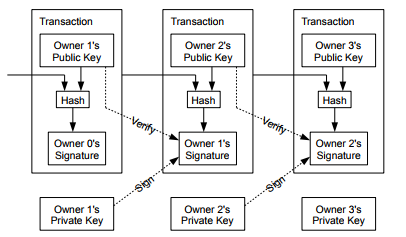
\includegraphics{./figs/transaction.png}
   \caption{Modelo de transa\c{c}\~oes com encadeamento de propriedade}
   \label{fig:transaction}
 \end{center}
\end{figure}

De fato, todas as bitcoins podem ter seus tra\c{c}os perseguidos ao longo de todas as transa\c{c}\~oes em que estiveram envolvidas, visto que todos os n\'os da rede operam com uma c\'opia fiel do mesmo livro raz\~ao. Ao final, sempre encontra-se o bloco em que tenham sido mineradas. Cada moeda que ainda n\~ao foi gasta tem sua origem na sa\'ida de uma transa\c{c}\~ao - UTXO.

\subsection{Cadeia de Blocos}

A solu\c{c}\~ao proposta por \citeonline{bitcoin} requer a utiliza\c{c}\~ao de um sistema distribu\'ido de \textit{timestamp}, pois assim prova-se que os dados existiram num determinado momento.
Desta forma, cada transa\c{c}\~ao ocorre numa data e hora espec\'ifica e assim que for publicada na rede ficar\'a em estado pendente.
Para ser confirmada, a transa\c{c}\~ao deve ser inclu\'ida num bloco v\'alido encontrado por um n\'o mineiro.
Um bloco \'e uma estrutura de dados que possui como informa\c{c}\~ao principal um conjunto de transa\c{c}\~oes.
Para que o sistema de \textit{timestamp} funcione, cada bloco possui o \textit{hash} do bloco anterior, formando uma lista encadeada.
A figura \ref{fig:blockchain} ilustra o processo.

\begin{figure}[ht]
 \begin{center}
   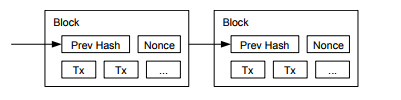
\includegraphics[width=90mm,scale=1.0]{./figs/blockchain.png}
   \caption{Modelo da blockchain}
   \label{fig:blockchain}
 \end{center}
\end{figure}

O processo de descoberta de novos blocos, tamb\'{e}m chamado de minera\c{c}\~{a}o e respons\'avel por garantir consenso entre todos os n\'os, ocorre atrav\'es de um algoritmo de for\c{c}a bruta como PoW.
Tal algoritmo tenta exaustivamente encontrar um valor (\textit{nonce} - inclu\'ido na estrutura do bloco) at\'e que o \textit{hash} do bloco comece com um n\'umero espec\'ifico de bits zero, definido dinamicamente pela rede.
Quanto mais bits requeridos, mais dif\'icil se torna a minera\c{c}\~ao e, com isso, a rede ajusta-se naturalmente ao aumento ou diminui\c{c}\~ao do total de processamento (medido em \textit{hashrate}) fornecido pelos mineiros.
Em m\'edia, a dificuldade \'e exponencial \`a quantidade de bits requisitados.
Assim, a altera\c{c}\~ao de um bloco j\'a inserido na rede necessariamente implica na realiza\c{c}\~ao deste trabalho novamente, inclusive para os blocos que o sucedem, visto que o \textit{hash} de cada bloco \'e inclu\'ido em seu sucessor, refor\c{c}ando a seguran\c{c}a da rede a cada itera\c{c}\~ao \cite{bitcoin}.

Para economizar espa\c{c}o de disco e agilizar o processo de sincroniza\c{c}\~ao com a rede, o bloco inclui a raiz da \'arvore de assinaturas ~\cite{merkle} de suas transa\c{c}\~oes. Isto possibilita a verifica\c{c}\~ao de pagamentos de forma confi\'avel (desde que n\'os honestos sejam maioria da rede) sem despender processamento de verifica\c{c}\~ao individual de cada transa\c{c}\~ao, pois a raiz da \'arvore - Merkle Root, um \textit{hash} - est\'a integrada ao \textit{hash} do bloco.

\subsection{Minera\c{c}\~ao}

Por conven\c{c}\~ao, a primeira transa\c{c}\~ao de um novo bloco coloca em circula\c{c}\~ao novas bitcoins, em posse daquele que o encontrou.
Trata-se de uma recompensa\footnote{Ou custo, a depender da perspectiva. Na emiss\~ao de novas moedas a cada bloco, existe uma taxa de infla\c{c}\~ao matematicamente previs\'ivel que independe do volume de \textit{hashrate}. Desta forma, a comunidade coletivamente custeia um sal\'ario pelo servi\c{c}o de mineiro.} para que os n\'os continuem a prover a seguran\c{c}a necess\'aria da rede de forma honesta.
Por\'em, o montante cai pela metade em intervalos de 210 mil blocos, at\'e que todas as bitcoins sejam mineradas at\'e o limite de 21 milh\~oes\footnote{Vale ressaltar que existem muitas bitcoins perdidas, pois uma vez que se perde o controle de sua chave privada, voc\^e fica impossibilitado de utiliz\'a-las.
Al\'em disso, estima-se que um grande montante de bitcoins originados nos primeiros meses da rede, sob controle de Satoshi Nakamoto, n\~ao ser\~ao jamais utilizados.
Portanto, na pr\'atica, o montante em circula\c{c}\~ao ser\'a inferior ao limite.} \cite{bitcoin}.

Um n\'o mineiro tem duas responsabilidades: validar o conte\'udo das transa\c{c}\~oes que aguardam serem inclu\'idas num bloco e rodar o processo de minera\c{c}\~ao que \'e a \'unica maneira de se descobrir novos blocos.
As transa\c{c}\~oes que ainda n\~ao foram verificadas e inseridas num bloco ficam pendentes numa fila e podem receber prioridade pelos mineiros de acordo com a quantidade despendida em taxas.
As taxas de transa\c{c}\~ao ser\~ao a \'unica forma de receita dos mineiros quando todas as bitcoins j\'a estiverem em circula\c{c}\~ao.

\'{E} importante notar que a verifica\c{c}\~{a}o criptogr\'{a}fica do conte\'{u}do da \textit{blockchain} n\~{a}o \'e t\~ao computacionalmente exigente quanto a minera\c{c}\~ao.
O funcionamento do algoritmo que \'{e} utilizado como PoW no Bitcoin para minera\c{c}\~{a}o, este sim extremamente dispendioso, torna aleat\'{o}ria a escolha do mineiro a descobrir o pr\'{o}ximo bloco da cadeia.
Quanto maior o \textit{hashrate} disponibilizado por um mineiro, maior a probabilidade dele encontrar um bloco v\'{a}lido a ser aceito pela rede.
A seguran\c{c}a dos dados da \textit{blockchain} \'e diretamente proporcional \`a quantidade total de \textit{hashrate} na rede. A competi\c{c}\~{a}o por maiores fatias do \textit{hashrate} total provido para a rede, que visa o ac\'umulo da moeda emitida em cada bloco, \'{e} importante para garantir a integridade e honestidade de pelo menos 51\% deste, sendo a solu\c{c}\~{a}o encontrada por \citeonline{bitcoin} para resolver o problema dos generais bizantinos nesta rede \cite{byzantium}.

\section{Ethereum}

A chamada segunda gera\c{c}\~ao de criptomoedas surgiu com a proposta de utilizar-se da seguran\c{c}a provida por uma \textit{blockchain} na constru\c{c}\~ao de protocolos mais complexos, servindo como uma camada fundamental \cite{survey}.
Para tal, \'e necess\'ario ir al\'em do sistema de transa\c{c}\~oes do Bitcoin que oferece recursos limitados em seus \textit{scripts} de transa\c{c}\~oes, que basicamente descrevem regras para que o receptor consiga ganhar acesso \`as moedas.

Para possibilitar casos de usos mais elaborados obtidos ao explorar-se conceitos como o de contrato inteligente \cite{smartcontract}, Ethereum \'e um protocolo que objetiva fornecer aos desenvolvedores uma linguagem de programa\c{c}\~ao Turing-completa \cite{ethereum}.
A falta de artif\'icios como \textit{loops} na linguagem de \textit{scripting} do Bitcoin impossibilita a escrita de muitos tipos de contratos\footnote{Entretanto, trata-se de um experimento em andamento. A proposta de melhoria do Bitcoin (BIP) 141, adotada em consenso e conhecida como SegWit \cite{segwit}, faz com que o versionamento seja levado em conta num \textit{script}. Isto remove a necessidade de um \textit{hardfork} para novas atualiza\c{c}\~oes da linguagem.}, assim como a simplicidade do estado bin\'ario atribu\'ido a uma UTXO - despendida ou n\~ao  \cite{utxodan}.

Uma \textit{blockchain} pode ser vista como sendo um sistema de transi\c{c}\~oes.
O estado atual \'e computado atrav\'es de uma fun\c{c}\~ao que recebe como entrada um estado e uma transa\c{c}\~ao e gera como sa\'ida um novo estado.
Tal fun\c{c}\~ao pode ser deliberadamente escrita na forma de um contrato em alguma das linguagens de alto n\'ivel suportadas como a Solidity, sendo o c\'odigo resultante executado na EVM.
O custo computacional para executar o c\'{o}digo de um contrato pelos mineiros \'{e} pago pelo usu\'{a}rio e deduzido do n\'{u}mero de itera\c{c}\~{o}es necess\'{a}rias na EVM sendo incluso na transa\c{c}\~{a}o os campos \textit{startgas} (o n\'{u}mero m\'{a}ximo de itera\c{c}\~{o}es) e \textit{gasprice} (o valor despendido pelo usu\'{a}rio para cada uma).
Desta forma evita-se ataques de \textit{spam} como no caso de um \textit{loop} infinito no c\'{o}digo de um contrato \cite{ethreview}.

Ao contr\'ario do Bitcoin, a infla\c{c}\~ao no protocolo Ethereum n\~ao possui um limite superior. Os mineiros continuar\~ao colocando cada vez mais moedas em circula\c{c}\~ao \cite{ethereumissuance}.
Preocupados com a escalabilidade do protocolo, os desenvolvedores da Ethereum Foundation enveredaram por uma linha de pesquisa onde pretendem atualizar o mecanismo de consenso para PoS \cite{casper}.
Tamb\'em pretendem adotar os conceitos da Lightning Network do ecossistema Bitcoin via Raiden Network, onde a ideia fundamental \'e escalar o sistema para camadas \textit{off-chain} de computa\c{c}\~ao de forma a minimizar o uso da \textit{blockchain} que torna-se apenas a camada fundamental para assentamento do estado das opera\c{c}\~oes realizadas nos chamados \textit{state channels} \cite{plasma}.

\subsection{Contrato Inteligente}
\citeonline{smartcontract} sugere que muitos tipos de contratos podem ser embutidos em \textit{hardware} e \textit{software}.
O exemplo mais simples \'{e} a m\'{a}quina de vendas, onde o interessado insere dinheiro na entrada da mesma que fica a cargo da gest\~{a}o de seus recursos dispon\'{i}veis.
Para tanto, as regras contidas em seu programa equivalem a cl\'{a}usulas contratuais.

Al\'em de moedas, a aplicabilidade \'e diversa.
Por exemplo, contratos podem ser utilizados para a cria\c{c}\~ao de \textit{dapps} como derivativos e outros t\'itulos financeiros, sistemas de reputa\c{c}\~ao e identidade, armazenamento de arquivos, conta-poupan\c{c}a, testamento, etc \cite{ethereum}.
Pode-se, inclusive, botar em pr\'atica o conceito de Empresa Aut\^omata Descentralizada (DAC) \cite{dac}\footnote{No dia 25 de Julho de 2017, a SEC dos Estados Unidos emite uma nota dizendo que determinado conjunto de leis estadunidenses poderia ser extendido \`a organiza\c{c}\~oes virtuais.
Um ano antes, uma falha foi explorada no contrato inteligente TheDAO na rede Ethereum que permitiu o desvio das moedas acumuladas pelo mesmo, gerando preju\'izo avaliado em mais de 100 milh\~oes de d\'olares e um \textit{hardfork} na rede.}.
Abaixo um exemplo de o que talvez seja o contrato mais simples poss\'ivel de se implementar em Solidity para Ethereum:

\lstset{tabsize=5,language=javascript,showstringspaces=false,basicstyle=\ttfamily\small,keywordstyle=\bf,breaklines=true}
\begin{singlespacing}
\begin{lstlisting}[frame=single,framexrightmargin=1pt,numbers=left]
pragma solidity ^0.4.22;
contract hello_world {
 function render () public pure returns (string) {
   return 'hello world';
 }
}
\end{lstlisting}
\end{singlespacing}

Em qualquer neg\'{o}cio existem, basicamente, dois grupos de indiv\'{i}duos: aqueles que produzem valor e aqueles que o consomem.
Por\'{e}m, \'{e} muito comum, no contexto do paradigma centralizado, que as partes envolvidas possuam interesses desalinhados por serem intermediadas pelo dono do neg\'ocio.
O acionista zela pelo lucro, pela sa\'{u}de financeira da empresa e tem particular interesse em relat\'{o}rios e balan\c{c}os peri\'{o}dicos, etc.
O produtor tamb\'{e}m visa a maximiza\c{c}\~{a}o de seu lucro mas depende diretamente do tempo que disp\~oe para obt\^e-lo.
Em contrapartida, o usu\'{a}rio n\~{a}o se importa com o neg\'{o}cio em si e apenas espera uma plataforma de f\'{a}cil uso, eficiente e barata.

Ao modelar um neg\'{o}cio de forma descentralizada atrav\'{e}s de contratos inteligentes, os interesses de todas as partes se alinham.
Afinal, a pr\'{o}pria empresa e todo seu capital pode ser representada pelos \textit{tokens} criados, criando assim um la\c{c}o econ\^omico entre o produtor e o usu\'ario.
Al\'{e}m de n\~{a}o precisarem mais pagar uma ou v\'arias taxas de intermedia\c{c}\~ao (definidas pelo acionista) por n\~{a}o serem os donos dos meios de produ\c{c}\~{a}o, os usu\'{a}rios s\~{a}o inclu\'{i}dos no modelo fechando, assim, um ciclo econ\^{o}mico eficiente onde todos s\~{a}o como \textit{shareholders} - ou \textit{tokenhodlers}.

\section{EOSIO}

Um dos maiores debates em pauta nas comunidades das maiores \textit{blockchains} que adotam PoW como mecanismo de consenso gira em torno da escalabilidade do sistema.
Originalmente, \citeonline{bitcoin} prop\^os uma solu\c{c}\~ao linear tempor\'aria que \'e o aumento da capacidade de cada bloco via um \textit{hardfork}.
Entretanto, novos mecanismos ganharam destaque, principalmente ap\'os a segunda gera\c{c}\~ao de \textit{blockchains}.

Surgiu em 2012 a Peercoin, com a ideia de construir uma \textit{blockchain} segura sem que houvesse enormes gastos com energia el\'etrica como acontece na minera\c{c}\~ao em redes PoW\footnote{Estima-se que, anualmente, os mineiros em conjunto gastem bilh\~oes de d\'olares com custos de energia el\'etrica. Trata-se de uma infla\c{c}\~{a}o velada.} - como visto no comparativo da figura \ref{fig:energy}.
O mecanismo de consenso PoS foi proposto, embora na pr\'atica os desenvolvedores optaram por implementar um mecanismo h\'ibrido PoW/PoS.
As dificuldades que enfrentaram na tentativa de usar apenas PoS s\~ao explicadas por diversos cr\'iticos do mecanismo, como \citeonline{longrange}.

\begin{figure}[ht]
 \begin{center}
   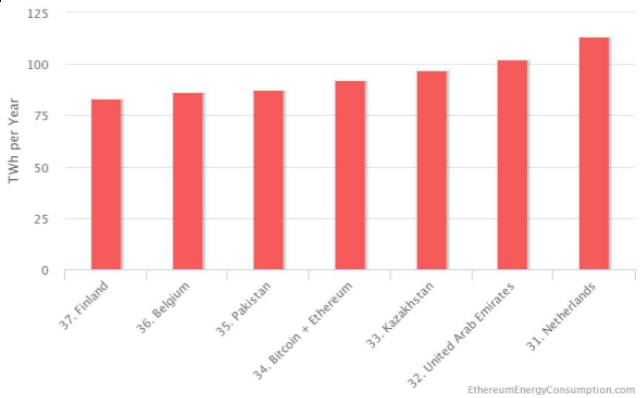
\includegraphics[width=120mm,scale=1.0]{./figs/energy.png}
   \caption{Consumo das redes BTC e ETH\footnotemark}
   \label{fig:energy}
 \end{center}
\end{figure}

\footnotetext{Mineiros em conjunto, comparados com o consumo individual de eletricidade de outros pa\'ises. Dispon\'ivel em: \url{https://digiconomist.net/ethereum-energy-consumption} (acesso em 17/11/2018).}

Existem diversas varia\c{c}\~oes do PoS, sendo que a diferen\c{c}a principal esteja na forma de selecionar o pr\'oximo n\'o a validar e inserir um novo bloco.
Em sua forma mais simples, quanto maior o \textit{stake}, isto \'e, o montante de \textit{tokens} em posse de um n\'o, maiores as chances dele ser escolhido para validar o pr\'oximo bloco \cite{pos}.
Pode-se tra\c{c}ar uma analogia com o sistema lot\'{e}rico onde cada moeda corresponde a um bilhete e, portanto, quanto mais bilhetes maior a probabilidade de acerto\footnote{Desde que consenso deve ser necessariamente atingido pela maioria dos participantes da rede, a analogia com o voto tamb\'em \'e v\'alida. Em redes PoW, um voto equivale a uma unidade de \textit{hashrate} e em redes PoS, um voto equivale a uma unidade do \textit{token}}.

Indo mais al\'em, o mecanismo DPoS parte do princ\'ipio de que os BPs (an\'{a}logos aos mineiros) devem ser eleitos\footnote{Tecnicamente, qualquer pessoa pode competir para minerar um bloco na rede Bitcoin, mas na pr\'atica existe uma grande centraliza\c{c}\~ao do \textit{hashrate}, que fica sob controle majorit\'ario de poucas grandes empresas.}.
Desta forma, um n\'o ganha ou perde fun\c{c}\~ao de validador atrav\'es do voto da comunidade \cite{dpos}.
Isto possibilita muitas otimiza\c{c}\~oes, visto que enquanto o \textit{throughput} de transa\c{c}\~oes por segundo suportado por redes PoW esteja limitado a poucas dezenas na melhor hip\'otese e o pr\'oximo bloco a ser minerado n\~ao possui \textit{timestamp} previs\'ivel (podendo chegar a horas de intervalo, a depender da estabilidade da rede), \textit{blockchains} que adotam DPoS possuem capacidade para milhares com intervalo entre blocos fixado \cite{bitshares}, sendo de apenas meio segundo em EOSIO.

Ap\'os o \^exito no \textit{bootstrap} de ambos os projetos Bitshares e Steemit, respectivamente uma \textit{exchange} e uma rede social descentralizadas, \citeonline{eos} divulga em Maio de 2017 seu novo projeto: EOSIO.
A proposta de uma nova arquitetura de \textit{blockchain} idealiza atingir escalabilidade horizontal e vertical para \textit{dapps}.
Diferentemente do protocolo Ethereum, EOSIO apresenta uma arquitetura que independe de uma implementa\c{c}\~{a}o espec\'{i}fica de m\'{a}quina virtual e o custo da valida\c{c}\~ao das transa\c{c}\~oes \'{e} coberto pela infla\c{c}\~{a}o anual definida pela constitui\c{c}\~{a}o, destinada em parte para incentivar os produtores de blocos.
Ao possuir os \textit{tokens}, o usu\'{a}rio possui o direito de realizar transa\c{c}\~{o}es livremente, proporcionalmente ao seu \textit{stake} e, desta forma, introduz-se um modelo eficiente sem a necessidade de taxas de transa\c{c}\~{a}o como em \textit{chains} PoW, que pode inclusive gerar problemas com o fisco em muitos pa\'{i}ses.

Por utilizar nativamente contratos compilados em WebAssembly, o desenvolvimento de \textit{dapps} poder\'{a} ser feito em m\'{u}ltiplas linguagens.
Abaixo um exemplo de como seria uma fun\c{c}\~{a}o de transfer\^{e}ncia implementada em C++ no contexto de um b\'{a}sico tipo de contrato: uma moeda (\textit{token}) \footnote{Dispon\'{i}vel em: \url{https://github.com/EOSIO/eosio.contracts/blob/master/eosio.token/src/eosio.token.cpp#L87} (acesso em 17-11-2018).}.

\lstset{tabsize=5,language=C++,showstringspaces=false,basicstyle=\ttfamily\small,keywordstyle=\bf,breaklines=true}
\begin{singlespacing}
\begin{lstlisting}[frame=single,framexrightmargin=1pt,numbers=left]
void token::transfer( name    from,
                      name    to,
                      asset   quantity,
                      string  memo )
{
     eosio_assert( from != to, "cannot transfer to self" );
     require_auth( from );
     eosio_assert( is_account(to), "to account does not exist" );
     auto sym = quantity.symbol.code();
     stats statstable( _self, sym.raw() );
     const auto& st = statstable.get( sym.raw() );

     require_recipient( from );
     require_recipient( to );

     eosio_assert( quantity.is_valid(), "invalid quantity" );
     eosio_assert( quantity.amount > 0, "must transfer positive quantity" );
     eosio_assert( quantity.symbol == st.supply.symbol, "symbol precision mismatch" );
     eosio_assert( memo.size() <= 256, "memo has more than 256 bytes" );

     auto payer = has_auth( to ) ? to : from;

     sub_balance( from, quantity );
     add_balance( to, quantity, payer );
}

\end{lstlisting}
\end{singlespacing}

Ao combinar elevado \textit{throughput} com conveni\^{e}ncias para seu p\'{u}blico-alvo, os desenvolvedores, EOSIO permite a cria\c{c}\~{a}o de aplica\c{c}\~{o}es atualmente impratic\'{a}veis no contexto de qualquer outra \textit{blockchain}.
Fora que a distribui\c{c}\~ao da emiss\~ao da moeda \'e mais uniforme, como verificado na figura \ref{fig:eosbp}.

\begin{figure}[ht]
 \begin{center}
   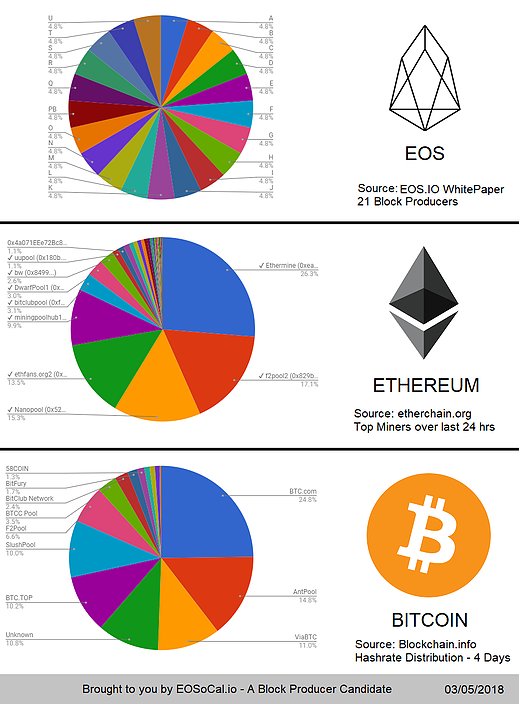
\includegraphics[width=100mm,scale=0.7]{./figs/eos-bp-distribution.png}
   \caption{Diferen\c{c}a na distribui\c{c}\~ao de validadores entre DPoS e PoW\footnotemark}
   \label{fig:eosbp}
 \end{center}
\end{figure}

\footnotetext{Dispon\'ivel em: \url{https://eossocal.io/} (acesso em 17-11-2018).}

\subsection{Governan\c{c}a}
Uma caracter\'istica do projeto \'e a tentativa em incluir aspectos governamentais numa \textit{blockchain}.
Ao contr\'ario de protocolos onde se firma na ideia de que o c\'odigo-fonte \'e lei, EOSIO \'e a primeira \textit{blockchain} a fazer uso de Contratos Ricardianos \cite{ricardian}.
Nestes, os desenvolvedores conseguem delinear a inten\c{c}\~ao de seus programas de forma que, em caso de \textit{bug} ou disputa entre terceiros, o mesmo sirva como um regulamento para consenso \cite{intentofcode}.

Fato \'e que, mesmo informalmente, processos mais ou menos definidos de governan\c{c}a existem em todas as \textit{blockchains}.
Permiss\~oes de escrita em reposit\'orios, qual vers\~ao rodar, quais ideias implementar e o que fazer em caso de \textit{bugs} s\~ao alguns exemplos de situa\c{c}\~oes em que deve haver consenso dos participantes da rede, mesmo que sem um processo de tomada de decis\~ao bem definido \cite{decentgovern}.
Em momentos de crise como na ocasi\~{a}o em que o Ethereum Classic (ETC) foi criado atrav\'{e}s de um \textit{hardfork} do Ethereum, uma decis\~{a}o dr\'{a}stica por conta de um \textit{bug}\footnote{No contrato TheDAO.} teve de ser tomada e os participantes da rede simplesmente n\~{a}o possu\'{i}am os meios para faz\^{e}-la consensualmente de forma descentralizada.
O resultado surgiu atrav\'{e}s do voto da Ethereum Foundation.
O grupo discordante se viu for\c{c}ado a separar-se na cria\c{c}\~{a}o de uma rede independente, uma solu\c{c}\~{a}o longe do ideal.
Tais \textit{forks} contingentes, em sua maioria originados na diverg\^encia de opini\~oes, tamb\'em aconteceram por diversas vezes na rede Bitcoin.

A tomada de decis\~ao em \textit{blockchains} EOSIO \'e feita por via de vota\c{c}\~ao por aprova\c{c}\~ao \cite{approvalvoting} onde um \textit{token} equivale a um voto.
Cr\'iticos desse sistema afirmam que a compra de votos inevitavelmente faria o protocolo se degradar para uma plutocracia \cite{plutocracy}.
Mas, tomando-se a figura de uma \textit{blockchain} ser an\'aloga \`a uma esta\c{c}\~ao de r\'adio, em que pessoas escutam e transmitem, temos que:

\begin{enumerate}
\item Em sistemas PoW como Bitcoin e Ethereum, para definir quem possui a permiss\~ao de transmitir parte-se do crit\'erio de quem consiga transmitir com maior pot\^encia.
\item Em sistemas PoS, exclui-se a necessidade de uma esta\c{c}\~ao grande o suficiente para anular o sinal dos demais. Por\'em, o requisito t\'ecnico de opera\c{c}\~ao ainda existe.
\item Em sistemas DPoS, a comunidade escolhe quais esta\c{c}\~oes ter\~ao permiss\~ao de transmitir. 
\end{enumerate}

Trata-se de uma abordagem que aproxima a tomada de decis\~ao a um processo democr\'atico.
\'E poss\'ivel que atores maliciosos consigam obter o controle de 51\% dos votos, mas h\'a de se levar em considera\c{c}\~ao o custo da compra destes \textit{tokens} al\'em de que, em \'ultima inst\^ancia, um \textit{hardfork} continua sendo uma op\c{c}\~ao \cite{radio}.

Em \textit{blockchains} EOSIO, necessita-se de ao menos (2/3)+1 dos BPs para se obter consenso.
Na principal rede fazendo uso do protocolo, EOS, conta-se com um grupo de 21 BPs que \'e mantido em xeque atrav\'es do poder do voto da comunidade.
Esta tamb\'em pode exigir que BPs atualizem seus n\'os com modifica\c{c}\~oes do sistema via referendo\footnote{E.g. \url{https://eosvotes.io/} (acesso em 17-11-2018).} (at\'e o momento, diversas atualiza\c{c}\~oes menores j\'a foram implementadas, bastando a autoriza\c{c}\~ao de 15 BPs).
Al\'em disso, a constitui\c{c}\~ao a que todos os usu\'arios da rede ficam submetidos prev\^e pelo menos um f\'orum de arbitragem (ECAF), onde disputas s\~ao submetidas para orientar a decis\~ao dos BPs.
Casos recentes onde fundos ou contas roubados conseguiram retornar a seus donos originais sugerem a aplicabilidade de governan\c{c}a mais pr\'oxima da realidade\footnote{Qualquer usu\'ario pode abrir uma disputa em \url{https://eoscorearbitration.io/} (acesso em 17-11-2018).}.
Pessoas comuns n\~ao ir\~ao adotar esta nova tecnologia em suas vidas se perder tudo, de forma irrevers\'ivel, esteja a dist\^ancia de um clique - como em outras \textit{blockchains}.

\section{Considera\c{c}\~oes Finais}

O protocolo Bitcoin possui grande capacidade de resili\^{e}ncia a ataques diversos e censura, o que justifica sua crescente ado\c{c}\~{a}o.
Por representar uma alternativa \`{a} oligop\'{o}lios seculares de reserva fracion\'aria, a tecnologia conhecida como \textit{blockchain} inventada por \citeonline{bitcoin} \'{e} o embri\~{a}o necess\'{a}rio para a cria\c{c}\~{a}o e manuten\c{c}\~{a}o de mercados mais livres, com um vi\'{e}s comunit\'{a}rio onde os pr\'{o}prios participantes s\~{a}o os respons\'{a}veis pela gera\c{c}\~{a}o de valor.

Ao se explorar inova\c{c}\~{o}es al\'{e}m do Bitcoin como o protocolo Ethereum, fica n\'{i}tido como novas formas de organiza\c{c}\~{o}es socioecon\^{o}micas poder\~{a}o surgir a partir do conceito fundamental de descentraliza\c{c}\~{a}o e \textit{tokeniza\c{c}\~{a}o}.
Tal demanda, por si s\'{o}, tamb\'{e}m indica o grave problema de escalabilidade atualmente em discuss\~{a}o.

Por conta disso, o projeto EOSIO tem como mote a ideia de "descentralizar tudo", promovendo recursos e alta performance para suprir a demanda de desenvolvedores de \textit{dapps}.
Comunidades de servi\c{c}os descentralizados que competir\~ao com suas contrapartes centralizadas como Uber, Airbnb, Spotify, Github e muitos outros poder\~ao tomar forma ao utilizarem o \textit{software} \cite{eos_intro}.

\chapter{Revis\~{a}o da Literatura}

Este cap\'{i}tulo traz um levantamento acerca dos problemas enfrentados por desenvolvedores de \textit{dapps} e alguns exemplos de como foram solucionados.
Primeiramente, conceitos b\'asicos sobre pseudoaleatoriedade s\~ao colocados para, ent\~ao, analisar-se m\'etodos para se obter entropia numa \textit{blockchain}. Por fim, diversos exemplos sao abordados.

\section{Pseudoaleatoriedade}

A demanda por n\'{u}meros aleat\'orios engloba uma ampla gama de aplica\c{c}\~{o}es, n\~{a}o sendo exclusiva aos jogos.
Al\'{e}m desta, diversas outras \'{a}reas empregam seu uso como por exemplo na estat\'{i}stica, criptografia e simula\c{c}\~{o}es computacionais.
Apesar de a aplica\c{c}\~ao da aleatoriedade em si tenha se iniciado mil\^enios atr\'as em m\'etodos divinat\'orios (e.g. Tar\^o, I-Ching, astragalomancia, etc), os primeiros avan\c{c}os de estudo formal surgiram com Cardano, Galileu e Pascal.

Entretanto, torna-se necess\'{a}rio realizar uma distin\c{c}\~{a}o importante.
Verdadeira aleatoriedade \'{e} imposs\'{i}vel de ser alcan\c{c}ada de forma determin\'{i}stica \cite{neumann} e, portanto, existem duas formas b\'{a}sicas de se gerar n\'{u}meros aleat\'{o}rios: extraindo entropia natural do ambiente por via de capta\c{c}\~ao de ru\'idos externos como entrada (e.g. \textit{random.org} que utiliza-se de sensores atmosf\'ericos); ou atrav\'{e}s de algoritmos PRNG.

Nestes, um processo aritm\'{e}tico derivado do que ficou conhecido como m\'{e}todo Monte Carlo pode ser empregado para a resolu\c{c}\~{a}o do problema de gera\c{c}\~{a}o de n\'{u}meros aleat\'{o}rios uniformemente distribu\'{i}dos.
Trata-se de uma t\'{e}cnica de amostragem sofisticada muito \'{u}til em diversos problemas e ci\^{e}ncias.
O termo foi inicialmente cunhado por Ulam e Neumann, \`{a} \'{e}poca pesquisando bombas at\^{o}micas em Los Alamos, referenciando o antigo cassino localizado em M\^{o}naco.
\'{E} tamb\'{e}m citado como simula\c{c}\~{a}o estoc\'{a}stica por diversos autores \cite{montecarlo}.

A premissa \'{e} de que um conjunto de n\'{u}meros pseudoaleat\'{o}rios pode ser computado atrav\'{e}s de um conjunto inicial preestabelecido (semente) de n\'{u}meros uniformemente distribu\'{i}dos entre 0 e 1 \cite{johnson}.
J\'{a} eram realizados esfor\c{c}os de longa data nesse sentido, como por exemplo nas tabelas de \citeonline{tippett}, \citeonline{kendalsmith}, etc.

Uma consequ\^{e}ncia direta do determinismo do processo \'{e} a impossibilidade de evitar ciclos na \textit{stream} de n\'{u}meros.
Pela amostra (semente) possuir tamanho finito, a repeti\c{c}\~{a}o dos n\'{u}meros \'{e} garantida e a qualidade da sequ\^{e}ncia \'{e} diretamente proporcional ao tamanho do ciclo.
Isto foi minimizado por \citeonline{lehmer} ao propor o m\'{e}todo de congru\^{e}ncias, onde n\~{a}o existem pequenos ciclos imprevis\'{i}veis como em m\'{e}todos antecessores \cite{johnson}.
Os geradores congruentes lineares (LCG) s\~{a}o os mais conhecidos e seguem sendo os mais utilizados PRNGs (com diversas adapta\c{c}\~{o}es exploradas), pois s\~{a}o f\'{a}ceis de compreender e implementar, al\'{e}m de possuir execu\c{c}\~{a}o linear.
Abaixo um exemplo de implementa\c{c}\~{a}o em Python\footnote{Dispon\'{i}vel em: \url{https://en.wikipedia.org/wiki/Linear_congruential_generator} (acesso em 17-11-2018).}:

\lstset{tabsize=5,language=Python,showstringspaces=false,basicstyle=\ttfamily\small,keywordstyle=\bf,breaklines=true}
\begin{singlespacing}
\begin{lstlisting}[frame=single,framexrightmargin=1pt,numbers=left]
 def lcg(modulus, a, c, seed):
   while True:
     seed = (a * seed + c) % modulus
     yield seed
\end{lstlisting}
\end{singlespacing}

O m\'{e}todo \'{e} delineado pela vari\'{a}vel \textit{seed}. Formalmente, define-se um conjunto $X$ de n\'{u}meros pseudoaleat\'{o}rios da seguinte forma:

\begin{equation}
X_{n+1}=(aX_{n}+c) \bmod m
\label{eq:lcg}
\end{equation}

Na equa\c{c}\~{a}o acima, define-se um gerador Lehmer quando $c=0$ e um gerador congruente misto quando $c\neq0$.
Este \'{e} uma adapta\c{c}\~{a}o, que surgiu na d\'{e}cada de 60, daquele.
A distribui\c{c}\~{a}o inicial (semente) \'{e} denotada por $X_0$.
Uma boa maneira de visualizar o mecanismo \'{e} pensar na reta $y=ax+c$ sendo desenhada continuamente mas sendo modulada para trazer o tra\c{c}ado de volta para o quadrado $[0,m]$x$[0,m]$, como detalhado na figura \ref{fig:prng}\footnote{Dispon\'{i}vel em: \url{https://people.sc.fsu.edu/~jburkardt/classes/isc_2009/monte_carlo_sampling.pdf} (acesso em 17-11-2018).}.

\begin{theorem}
A sequ\^{e}ncia definida por $X$ possui per\'{i}odo completo (isto \'{e}, o ciclo \'{e} previsivelmente formado ap\'{o}s $m$ itera\c{c}\~{o}es, ponto de rein\'{i}cio da sequ\^{e}ncia)  se e somente se:
\begin{enumerate}
  \item o modulo $m$ e o incremento $c$ forem relativamente primos;
  \item $a-1$ for divis\'{i}vel por todos os fatores primos de $m$;
  \item $a-1$ for divis\'{i}vel por 4 se $m$ for divis\'{i}vel por 4.
\end{enumerate}
\end{theorem}

O teorema de \citeonline{hulldobell} exposto acima garante a exist\^{e}ncia de um subconjunto de permuta\c{c}\~{o}es entre $a$, $c$ e $m$ que implicam em per\'{i}odos maximizados. Desta forma, a qualidade da sequ\^{e}ncia ser\'{a} estat\'{i}sticamente satisfat\'{o}ria e capaz de ser aprovada em testes de aleatoriedade.

\begin{figure}[ht]
 \begin{center}
   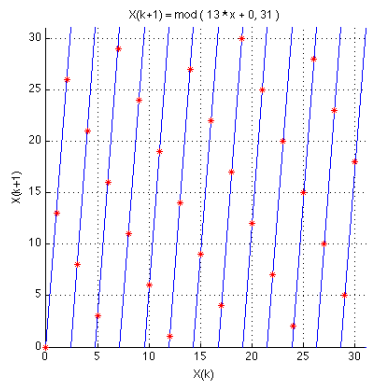
\includegraphics[width=90mm,scale=0.6]{./figs/prng.png}
   \caption{Inst\^{a}ncia de gerador congruente}
   \label{fig:prng}
 \end{center}
\end{figure}

\subsection{Entropia em Blockchains}
Existem quatro m\'{e}todos b\'{a}sicos atualmente sendo utilizados para a gera\c{c}\~{a}o de n\'{u}meros aleat\'{o}rios no contexto de \textit{blockchains} \cite{ethrandom}:
\begin{enumerate}
\item
O primeiro e mais simples, por n\~{a}o despender muito processamento, consome a entropia inerente aos pr\'{o}prios dados da rede.
Quaisquer informa\c{c}\~{a}o contida no livro raz\~{a}o pode ser arbitrariamente utilizada para esta finalidade.
\item
Uma outra maneira surge ao utilizar um or\'{a}culo, um tipo de contrato inteligente, respons\'{a}vel por interagir com uma API externa (e.g. \textit{random.org}) capaz de fornecer grande entropia.
\item
Tamb\'em h\'{a} a ideia de combinar uma semente do cliente com uma do pr\'{o}prio contrato sendo executado.
Desta forma, uma \textit{string} aleat\'{o}ria enviada pelo cliente numa transa\c{c}\~{a}o \'{e} utilizada em conjunto de uma outra, enviada por algum outro cliente ou at\'e mesmo extra\'{i}da da \textit{blockchain} por via do primeiro m\'{e}todo pelo pr\'{o}prio contrato.
\item
Por fim, \citeonline{neowiz} prop\~oe uma outra alternativa em que se utiliza uma assinatura criptogr\'afica como entropia.
Nele, o ator que requer o n\'umero aleat\'orio (\textit{revealer}) interage com o ator que o fornece (\textit{committer}) atrav\'es de um contrato inteligente, como explicado na figura \ref{fig:neowiz}.
\end{enumerate}

\begin{figure}[ht]
 \begin{center}
   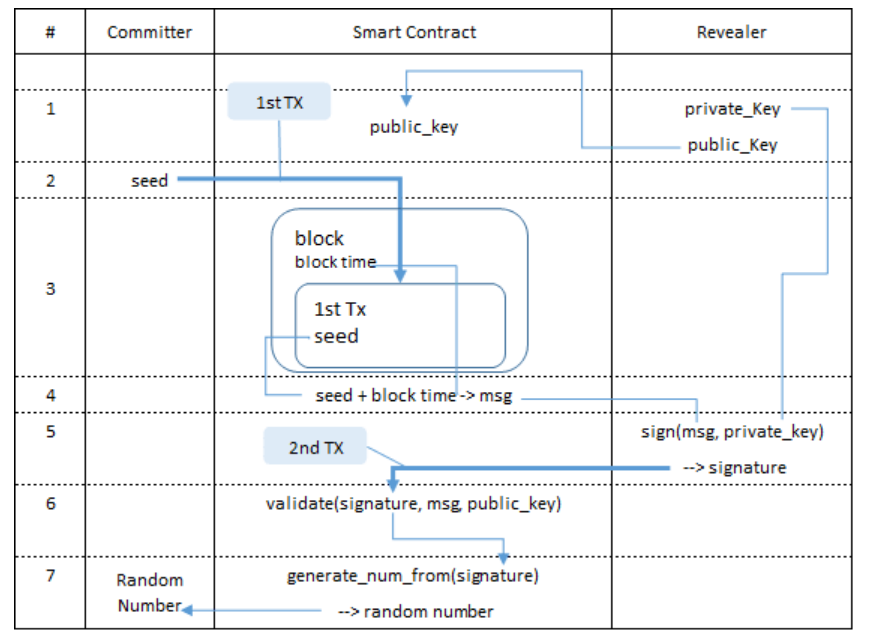
\includegraphics[width=120mm,scale=1.0]{./figs/neowiz.png}
   \caption[Modelo de PRNG em \textit{blockchains} via assinaturas]{Modelo de gera\c{c}\~ao de n\'umeros pseudoaleat\'orios via assinaturas criptogr\'aficas \cite{neowiz}}
   \label{fig:neowiz}
 \end{center}
\end{figure}

A escolha de um m\'{e}todo para uma aplica\c{c}\~{a}o espec\'{i}fica deve levar em conta algumas implica\c{c}\~{o}es.
Quanto ao primeiro, \'{e} importante considerar que toda e qualquer informa\c{c}\~{a}o contida numa \textit{blockchain} \'{e} de dom\'{i}nio p\'{u}blico e al\'{e}m disso pass\'{i}vel de \textit{front-running}\footnote{Uma vez que o mineiro tem total controle sobre quais transa\c{c}\~oes ser\~ao inclu\'idas num bloco, ele poderia escolher ignorar uma transa\c{c}\~ao vencedora, por exemplo.} pelos mineiros, n\~{a}o sendo poss\'{i}vel sua ado\c{c}\~{a}o em grande parte dos casos de uso com demanda por aleatoriedade.
Al\'em disso, em \textit{blockchains} que se utilizam do software EOSIO, por exemplo, n\~ao \'e poss\'ivel extrair dados como \textit{hashes} de blocos em contratos inteligentes.

O segundo garante, a princ\'ipio, uma excelente fonte de entropia mas o custo disso \'{e} a depend\^{e}ncia de um ator externo, aumentanto significativamente a centraliza\c{c}\~{a}o do sistema.
Afinal, situa\c{c}\~{o}es n\~{a}o raras de instabilidade num servidor central como o dispon\'{i}vel em \textit{random.org} e afins representam um grande risco para a previsibilidade e determinismo do sistema e, fora isso, \'{e} necess\'{a}rio depositar confian\c{c}a de que tal servi\c{c}o seja e continue sendo \'{i}ntegro e honesto.

Atinge-se no terceiro m\'etodo uma solu\c{c}\~{a}o mais confi\'{a}vel e pr\'{o}xima do ideal, por\'em a complexidade do sistema aumenta consideravelmente.
Corre-se o risco de reduzir a qualidade da experi\^encia de usu\'ario por conta disso e, de fato, a \'ultima t\'ecnica \'e a que mais vem sendo utilizada em \textit{dapps} atuais no ecossistema EOSIO.

\section{Aplica\c{c}\~{o}es Relacionadas}

Apesar do foco do presente trabalho seja a implementa\c{c}\~{a}o de um sistema descentralizado que funcione em \textit{blockchains} EOSIO, alguns dos exemplos citados nesta se\c{c}\~{a}o foram retirados de outras plataformas, por serem facilmente encontrados na literatura.

\subsection{Defini\c{c}\~ao de Dado Descentralizado}

O jogo mais simples que pode ser imaginado de forma descentralizada numa \textit{blockchain} com PoW como mecanismo de consenso simula o funcionamento de um dado virtual: ao apostar num determinado valor, o jogador ganha a partida caso o n\'{u}mero de \textit{threshold} aleatoriamente escolhido seja menor que aquele.
A probabilidade de ganhar uma partida \'{e} representado por \textit{p}, a quantia apostada por \textit{w} e \textit{h} representa a comiss\~{a}o do cassino virtual.
\citeonline{provablyfair} define o valor esperado de uma partida como:
\begin{equation}
EV = (h - 1)w
\label{eq:ev}
\end{equation}
Nota-se que o jogador garantidamente ir\'{a} perder uma pequena parte do montante a cada partida, visto que este \'{e} o mecanismo b\'{a}sico que garante o lucro de um cassino.
A quantia a ser recebida por um poss\'{i}vel ganhador \'{e} expressa como PV e o mesmo deve pagar PD em caso de derrota, trivialmente definido como -w.
Trata-se do valor em m\'{e}dia que o jogador pode esperar receber numa partida individual vitoriosa:
$$
EV=(1-p)PD+pPV
$$
Ao utilizar-se da equa\c{c}\~{a}o \ref{eq:ev}, vem:
$$
(h-1)w=(1-p)(-w)+pPV
$$
\begin{equation}
PV=\frac{wh}{p}-w
\label{eq:pv}
\end{equation}
Por fim, temos que a premissa fundamental \'{e} de que uma aposta vencedora ser\'{a} recompensada positivamente.
Portanto:
$$
PV>0
$$
Disto surge um novo limite ao dom\'{i}nio, quando utilizada a equa\c{c}\~{a}o \ref{eq:pv}:
$$
\frac{wh}{p}-w>0
$$
\begin{equation}
h>p
\label{eq:hp}
\end{equation}

A forma mais simples e direta de garantir imprevisibilidade para \textit{p} \'{e} utilizar dados da pr\'{o}pria \textit{blockchain}, como por exemplo o \textit{hash} de blocos e transa\c{c}\~{o}es.
Por\'{e}m, por serem informa\c{c}\~{o}es a princ\'{i}pio manipul\'{a}veis por n\'{o}s mineiros e potenciais atacantes, diversos cen\'{a}rios foram analisados extensivamente.
Conclui-se que um contrato inteligente numa rede PoW \'{e} o suficiente para garantir a seguran\c{c}a de um jogo como o descrito, para apostas onde $w \leq 1/h$ \cite{provablyfair}. 

\subsection{Exemplos de Dados}

A primeira \textit{dapp} a fazer uso da \textit{blockchain} Bitcoin para a implementa\c{c}\~ao de um jogo de dado foi anunciado em Abril de 2012, e continua em opera\c{c}\~ao nos dias de hoje.
SatoshiDICE utiliza o \textit{hash} da transa\c{c}\~ao em que o usu\'ario submete sua aposta em conjunto com uma semente que o mesmo desconhece para fabricar outro \textit{hash} SHA-512.
Os primeiros quatro \textit{bytes} configuram o n\'umero sorteado \cite{satoshidice}.

Etheroll \'e um contrato que simula um dado virtual na plataforma Ethereum.
O jogador envia uma transa\c{c}\~{a}o para a rede com o objetivo de executar a fun\c{c}\~{a}o \textit{playerRollDice(uint rollUnder)} do contrato, que fica a cargo de ent\~{a}o executar uma subconsulta ao servi\c{c}o especializado da \textit{random.org} atrav\'{e}s do or\'{a}culo implementado por \textit{oraclize.it}.
De maneira geral, o or\'{a}culo fica apenas respons\'{a}vel pela consuma\c{c}\~{a}o da API, como consta no \textit{script} da fun\c{c}\~{a}o\footnote{O c\'{o}digo fonte do contrato est\'a dispon\'ivel em: \url{https://etherscan.io/address/0xece701c76bd00d1c3f96410a0c69ea8dfcf5f34e\#code} (acesso em 17-11-2018).} \cite{etheroll}:

\lstset{tabsize=5,language=Python,showstringspaces=false,basicstyle=\ttfamily\small,keywordstyle=\bf,breaklines=true}
\begin{singlespacing}
\begin{lstlisting}[frame=single,framexrightmargin=1pt,numbers=left]
 /*
 * assign partially encrypted query to oraclize
 * only the apiKey is encrypted 
 * integer query is in plain text
 */        
 bytes32 rngId = oraclize_query("nested", "[URL] ['json(https://api.random.org/json-rpc/1/invoke).result.random[\"serialNumber\",\"data\"]', '\\n{\"jsonrpc\":\"2.0\",\"method\":\"generateSignedIntegers\",\"params\":{\"apiKey\":${[decrypt] BLTr+ZtMOLP2SQVXx8GRscYuXv+3wY5zdFgrQZNMMY3oO/6C7OoQkgu3KgfBuiJWW1S3U/+ya10XFGHv2P7MB7VYwFIZd3VOMI/Os8o1uJCdGGZgpR0Dkm5QoNH7MbDM0wa2RewBqlVLFGoZX1PJC+igBPNoHC4=},\"n\":1,\"min\":1,\"max\":100,\"replacement\":true,\"base\":10${[identity] \"}\"},\"id\":1${[identity] \"}\"}']", gasForOraclize);
\end{lstlisting}
\end{singlespacing}

No contexto EOSIO, a primeira \textit{dapp} de dado foi implementada pela EOSBet.
Apesar de terem lan\c{c}ado alguns prot\'otipos na Ethereum em 2017, consolidaram a decis\~ao de concentrar seus esfor\c{c}os em EOSIO.
Os motivos elencados pelos desenvolvedores condiz com o que foi falado neste trabalho.
Maior \textit{throughput}, inexist\^encia de taxas de transa\c{c}\~ao (melhorando, portanto, a experi\^encia dos usu\'arios) e maior facilidade de desenvolvimento s\~ao os principais.

\subsection{Exemplos de Loterias}
Uma plataforma que oferece uma loteria descentralizada, conhecida como Trueflip, recompensa apostas certeiras de n\'{u}meros num determinado intervalo.
Leva o pr\^{e}mio quem acertar 5 n\'{u}meros dentre 49 e 1 n\'{u}mero dentre 26.
Para a gera\c{c}\~{a}o aleat\'{o}ria dos n\'{u}meros sorteados, adota-se um processo que se baseia no primeiro m\'{e}todo abordado na \'{u}ltima se\c{c}\~{a}o.
Por defini\c{c}\~{a}o, o contrato decodifica o \textit{hash} do primeiro bloco v\'{a}lido que tenha sido minerado ap\'{o}s um \textit{timestamp} espec\'{i}fico, no protocolo Bitcoin.
Existe uma janela de tempo de forma que o cadastro de apostas se encerra antes deste momento \cite{trueflip}.
Por exemplo, ao considerar o \textit{hash} do bloco \#463346:

$0000000000000000001bf3b0a7fdf7e4889734f4f0c0cb00a1bb082cf3d4ad49$

Para a extra\c{c}\~{a}o de 6 n\'{u}meros, divide-se o final do \textit{hash} em segmentos de 4 caracteres.
Cada segmento $x_i$ \'{e} modulado e decodificado de hexadecimal para decimal:

$x_0=(f0c0)_{16} \bmod 49=(61632)_{10} \bmod 49=39$

$x_1=(cb00)_{16} \bmod 49=(51968)_{10} \bmod 49=28$

$x_2=(a1bb)_{16} \bmod 49=(41403)_{10} \bmod 49=47$

$x_3=(082c)_{16} \bmod 49=(2092)_{10} \bmod 49=34$

$x_4=(f3d4)_{16} \bmod 49=(62420)_{10} \bmod 49=43$

$x_5=(ad49)_{16} \bmod 49=(44361)_{10} \bmod 26=5$

Diferentemente da Trueflip, a loteria Kibo recolhe sementes geradas no \textit{frontend} da aplica\c{c}\~{a}o pelos jogadores no momento de compra dos bilhetes que garantem a participa\c{c}\~{a}o do jogo e os mistura com \textit{hashes} de blocos recentes.
Esta aplica\c{c}\~{a}o \'{e} peculiar pois sugere mecanismos de \textit{marketing} e governan\c{c}a n\~{a}o oferecidos nativamente pelo protocolo Ethereum.
Sendo na realidade um conjunto de contratos, Kibo define que a gest\~{a}o destes deva ser realizada \`{a} partir de decis\~{o}es tomadas por via de vota\c{c}\~{a}o de quem possui \textit{stake} do Control Token \cite{kibo}.

\subsection{Exemplos Diversos}

Um exemplo interessante \'{e} o contrato RANDAO, que objetiva fornecer n\'umeros aleat\'orios.
Nele, um esfor\c{c}o colaborativo \'{e} modelado num processo que envolve tr\^{e}s etapas\footnote{Explica\c{c}\~{a}o dispon\'{i}vel em: \url{https://github.com/randao/randao/blob/master/README.md} (acesso em 17-11-2018).}:

\begin{enumerate}
  \item Cole\c{c}\~{a}o de \textit{hashes sha3}: qualquer usu\'{a}rio interessado em participar na gera\c{c}\~{a}o de um n\'{u}mero aleat\'{o}rio envia ao contrato uma quantia $m$ de Ether como garantia e o resultado de $sha3(s)$, sendo $s$ um n\'{u}mero secreto escolhido arbitrariamente pelo mesmo como semente.
  \item Valida\c{c}\~{a}o das sementes: todos os participantes inclusos na primeira etapa devem agora enviar ao contrato suas respectivas sementes dentro de um per\'{i}odo de tempo previamente estipulado. O contrato faz a verifica\c{c}\~{a}o criptogr\'{a}fica e monta a cole\c{c}\~{a}o de sementes validadas.
  \item C\'{a}lculo do n\'{u}mero: ap\'{o}s a montagem da cole\c{c}\~{a}o, o contrato executa uma fun\c{c}\~{a}o $f(s_0,s_1,...,s_n)$ que resulta num n\'{u}mero aleat\'{o}rio que \'{e}, ent\~{a}o, enviado de volta para os participantes junto do valor $m+L$ em Ether. O lucro ($L$) do contrato ocorre das taxas paga por outros contratos ao solicitar aleatoriedade, que \'{e} ent\~{a}o dividido proporcionalmente \`{a} $m$ aos participantes do processo.
\end{enumerate}

Outro exemplo \'e a \textit{blockchain} Peerplays, que foi constru\'{i}da utilizando o \textit{software} Graphene (precursor do EOSIO, tamb\'em criado por Daniel Larimer) e, portanto, utiliza como mecanismo de consenso o DPoS.
Jogadores interagem com a plataforma atrav\'{e}s de contratos inteligentes e fazem uso de um PRNG embutido.
Para todo pr\^{e}mio recebido, a rede cobra uma pequena porcentagem que retorna como lucro para tr\^{e}s dire\c{c}\~{o}es.
A maior parte \'{e} destinada para todos os endere\c{c}os que possuem o \textit{token} nativo da plataforma como uma esp\'{e}cie de dividendo, outra parte para um fundo que arca com eventuais custos de desenvolvimento e resolu\c{c}\~{a}o de \textit{bugs} e por \'{u}ltimo um fundo a ser sorteado em frequentes Mega-Jackpots \cite{peerplays}.

Fora do contexto de cassinos, aplica\c{c}\~{o}es como FirstBlood e \citeonline{unikrn} idealizam a descentraliza\c{c}\~{a}o de apostas em partidas e torneios de \textit{eSports} como por exemplo League of Legends, DOTA 2 e Counter-Strike.
No caso da primeira, \'{e} proposto um sistema de verifica\c{c}\~{a}o de resultados pois a n\~{a}o ser que o jogo esteja rodando na EVM, ser\'{a} necess\'{a}rio um mecanismo de consenso para que os mesmos sejam inseridos na \textit{blockchain} Ethereum.
Para tanto, \'{e} preciso que no m\'{i}nimo duas testemunhas, que rodam \textit{software} especializado em conex\~{a}o com APIs centralizadas (tal como um or\'{a}culo) que fazem o \textit{broadcast} oficial das estat\'{i}sticas de uma partida, cheguem a um consenso do resultado.
Caso n\~{a}o seja poss\'{i}vel, um j\'{u}ri \'{e} formado para determinar o resultado original atrav\'{e}s de um sistema de vota\c{c}\~{a}o. 
O processo de sele\c{c}\~{a}o de testemunhas e componentes do j\'{u}ri \'{e} aleat\'{o}rio e requer \textit{stake} do \textit{token} nativo e al\'{e}m disso, para evitar ataques \textit{sybil} onde contas s\~{a}o criadas como \textit{spam} objetivando vantagens para o operador, a aplica\c{c}\~{a}o contar\'{a} com o suporte de um banco de dados centralizado onde s\~{a}o guardadas informa\c{c}\~{o}es de identidade dos agentes citados \cite{firstblood}.

Muitas \textit{dapps} v\^em surgindo no contexto EOSIO.
Alguns exemplos incluem a HireVibes\footnote{Dispon\'ivel em: \url{https://hirevibes.io/} (acesso em 17-11-2018).}, que \'e um aplicativo que permite que empregadores encontrem empregados;
Nougit\footnote{Primeiro lugar na EOS Global Hackathon em S\~ao Francisco, 12/11/2018.}, que \'e um sistema de gerenciamento de reposit\'orios git que faz uso de IPFS e valida os \textit{hashes} na \textit{blockchain};
e por fim a Everipedia\footnote{Dispon\'ivel em: \url{https://everipedia.org/} (acesso em 17-11-2018).}, que \'e uma concorrente da Wikipedia constru\'ida em EOSIO, que conta com um cofundador desta no time, Larry Sanger.

\section{Considera\c{c}\~oes Finais}

Apesar de possibilitar a implementa\c{c}\~{a}o de \textit{dapps} que rodam numa m\'{a}quina virtual distribu\'{i}da como a EVM, a efici\^{e}ncia da mesma \'{e} crucial na maior parte de casos de uso reais.
Caso modelado despreocupadamente com lenta computa\c{c}\~{a}o dos estados, um problema n\~{a}o ser\'{a} solucionado a ponto de ficar utiliz\'{a}vel, como verificado por \citeonline{chess} num jogo de xadrez que precisou passar por reformula\c{c}\~{o}es e recorrer \`{a} computa\c{c}\~{a}o \textit{off-chain} a cargo dos clientes para viabilizar seu uso na EVM; ou no caso da \textit{dapp} VGO que abandonou a Ethereum apenas 72 horas ap\'os seu lan\c{c}amento, tendo escolhido uma \textit{blockchain} DPoS para abrigar seu neg\'ocio \cite{wax}.

\chapter{Solu\c{c}\~{a}o Proposta}

Este cap\'itulo descreve a loteria proposta pelo presente trabalho.
Faz-se necess\'aria uma contextualiza\c{c}\~ao acerca do desenvolvimento e opera\c{c}\~ao de contratos com o protocolo EOSIO.
Na subse\c{c}\~ao seguinte, o funcionamento da loteria \'e visto em detalhes e, por fim, algumas considera\c{c}\~oes pertinentes s\~ao apresentadas.

\section{Contratos em EOSIO}

Para se desenvolver contratos para \textit{blockchains} EOSIO, uma SDK - ou CDT - foi criada\footnote{Dispon\'ivel em: \url{https://github.com/eosio/eosio.cdt/} (acesso em 17-11-2018).}.
O CDT auxilia os desenvolvedores ao fornecer uma s\'erie de ferramentas essenciais, como: biblioteca eosiolib, compilador\footnote{Clang modificado com suporte experimental a WebAssembly.} e gerador de ABI.
O exemplo mais simples de contrato como visto abaixo \'e compilado em um bin\'ario (WebAssembly), para que possa ser serializado e implantado numa \textit{blockchain}.

\lstset{tabsize=5,language=C++,showstringspaces=false,basicstyle=\ttfamily\small,keywordstyle=\bf,breaklines=true}
\begin{singlespacing}
\begin{lstlisting}[frame=single,framexrightmargin=1pt,numbers=left]
#include <eosiolib/eosio.hpp>

using namespace eosio;
using namespace std;

class [[eosio::contract("hello")]] hello : public contract
{
    public:
        using contract::contract;

        [[eosio::action]] void printact( string s )
        {
            print( s );
        }
};

EOSIO_DISPATCH( hello, (printact) )
\end{lstlisting}
\end{singlespacing}

Os atributos da biblioteca eosiolib ([[eosio::contract()]] e [[eosio::action]]) indicam ao gerador de ABI o que deve ser inclu\'ido.
Descrita em formato JSON, esta interface tamb\'em \'e implantada na \textit{blockchain} e serve como refer\^encia para que os n\'os da rede possam interagir com o contrato, al\'em de delinear o contrato Ricardiano para cada a\c{c}\~ao.
A macro EOSIO\_DISPATCH implementa a fun\c{c}\~ao \textit{apply}, que \'e chamada por \textit{default} pelos BPs na execu\c{c}\~ao de qualquer a\c{c}\~ao de um contrato.
Desta forma, abstrai-se o c\'odigo necess\'ario do protoco, que fica encapsulado, e um \textit{switch} interno encaminha o fluxo para o m\'etodo da a\c{c}\~ao, neste caso o \textit{printact}.
Al\'em da a\c{c}\~ao, a conta em que foi implantado o c\'odigo e a conta que autorizou a chamada fazem parte dos argumentos de \textit{apply}.

Para compilar e gerar a ABI do contrato utiliza-se os dois comandos:

\lstset{tabsize=5,language=sh,showstringspaces=false,basicstyle=\ttfamily\small,keywordstyle=\bf,breaklines=true}
\begin{singlespacing}
\begin{lstlisting}[frame=single,framexrightmargin=1pt,numbers=left]
% eosio-cpp -contract=hello -o=hello.wasm hello_world.cpp
% eosio-abigen -contract=hello -output=hello.abi hello_world.cpp
\end{lstlisting}
\end{singlespacing}

Isto feito, para se implantar o c\'odigo hello.wasm e sua ABI hello.abi, bem como para enviar outros comandos para os n\'os - ou \textit{nodeos} - da rede\footnote{Mais detalhes dispon\'iveis em: \url{https://developers.eos.io/} (acesso em 17-11-2018).}, \'e necess\'ario a utiliza\c{c}\~ao de uma interface de usu\'ario.
Essa interface consome uma API HTTP, arquitetada em RPC e exposta pelo \textit{nodeos}, sendo que a mais simples \'e a \textit{cleos} (CLI).
Ambos pertencem ao \textit{software} EOSIO\footnote{Dispon\'ivel em: \url{https://github.com/eosio/eos/} (acesso em 17-11-2018).}.

\begin{figure}[ht]
 \begin{center}
   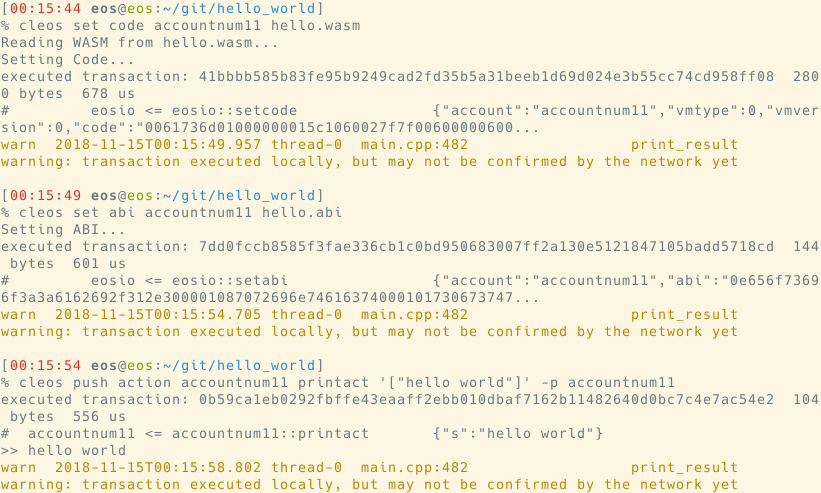
\includegraphics[width=160mm,scale=1.0]{./figs/cleos.png}
   \caption{Implanta\c{c}\~ao de um contrato e sua ABI}
   \label{fig:cleos}
 \end{center}
\end{figure}

As chamadas eosio::setcode\footnote{Novas vers\~oes do bin\'ario podem ser reimplantadas, efetivamente atualizando o c\'odigo do contrato que \'e dispon\'ivel para os n\'os da rede. Isto n\~ao \'e poss\'ivel na rede Ethereum.} e eosio::setabi s\~ao a\c{c}\~oes do contrato do sistema (\textit{eosio.system}).
Al\'em deste, outros integram o sistema como por exemplo \textit{eosio.token} (que implementa a moeda da rede) e \textit{eosio.msig} (\textit{multisig}, para que BPs autorizem a\c{c}\~oes em consenso).
Tanto as chamadas a a\c{c}\~oes, de qualquer contrato, quanto o \textit{output} destas s\~ao codificados em formato JSON, definindo assim uma mensagem.
Mensagens s\~ao trocadas pelos n\'os, que mant\'em o estado final da rede em mem\'oria e a depender de \textit{plugins} podem replicar o conte\'udo em bancos como MariaDB ou MongoDB.
Por possuir uma arquitetura modular, com \textit{plugins} para customizar o funcionamento do \textit{nodeos} e foco em contratos, os desenvolvedores optaram por desacoplar as funcionalidades b\'asicas da camada de consenso.

A\c{c}\~oes como criar novas contas, votar em BPs, delegar \textit{stake} e comprar ou vender mem\'oria RAM s\~ao algumas do \textit{eosio.system}.
Cada a\c{c}\~ao, ao ter sua mensagem transmitida, consome banda (NET). Quanto maior o tamanho da mensagem, mais dados ter\~ao que ser transferidos.
Al\'em da demanda de transmiss\~ao, existe a demanda por processamento em cada a\c{c}\~ao (CPU), a depender do m\'etodo que ela far\'a os BPs executarem.
Quanto maiores os \textit{stakes} (CPU ou NET) de uma conta autorizando a execu\c{c}\~ao de a\c{c}\~oes, mais recursos ela pode consumir.
Qualquer conta pode delegar CPU e NET para outras contas\footnote{\'E poss\'ivel, inclusive, emprestar recursos a outras contas usando \textit{dapps} como Chintai - \url{https://chintai.io/} (acesso em 17-11-2018). Uma solu\c{c}\~ao nativa num novo contrato de sistema est\'a previsto para uma pr\'oxima versao do EOSIO.}, sendo que o total \textit{staked} por uma conta define seus votos - caso ela tenha votado.

Um outro atributo da eosiolib \'e o [[eosio::table]], usado na defini\c{c}\~ao de tabelas que por sua vez s\~ao definidas em \textit{structs}.
Elas servem para que um contrato mantenha em mem\'oria o estado de seus dados\footnote{Por exemplo, o balan\c{c}o de moedas que uma conta possui \'e mantido numa tabela - a diferen\c{c}a fundamental para com o modelo UTXO.}.
Os contratos fazem leituras e escritas como num banco de dados, por via de \textit{containers} MultiIndex da biblioteca Boost.
Contratos tamb\'em podem ler tabelas de outros contratos, sendo que esta comunica\c{c}\~ao intercontratual deve ser considerada ass\'incrona.
Este modelo pode resultar em \textit{spam}, mas o algoritmo de limita\c{c}\~ao dos recursos resolve.
Segue um exemplo de tabela com apenas uma coluna e uma opera\c{c}\~ao de inser\c{c}\~ao para ilustrar:

\lstset{tabsize=5,language=C++,showstringspaces=false,basicstyle=\ttfamily\small,keywordstyle=\bf,breaklines=true}
\begin{singlespacing}
\begin{lstlisting}[frame=single,framexrightmargin=1pt,numbers=left]
struct [[eosio::table]] player
{
    name player;
    auto primary_key() const { return player.value; }
};
multi_index< name( "player" ), player > players;

[[eosio::action]] void insert( name row )
{
    players.emplace( _self, [&]( auto& p ) { p.player = row; } );
}
\end{lstlisting}
\end{singlespacing}

Chamar a a\c{c}\~ao \textit{insert} faz com que o contrato insira uma nova linha em sua tabela \textit{player} com o valor \textit{row}.
Al\'em de \textit{emplace}, diversos outros m\'etodos s\~ao fornecidos pela API MultiIndex como por exemplo o \textit{find} que serve para buscar um registro de acordo com a chave prim\'aria da tabela.
Outros \'indices tamb\'em podem ser criados numa mesma tabela, al\'em de ser poss\'ivel definir uma tabela com mais colunas - inclusive de outros tipos.

Enquanto n\~ao for removida, uma linha consumir\'a a quantidade necess\'aria de mem\'oria RAM de acordo com sua estrutura.
O c\'odigo do contrato tamb\'em \'e mantido em mem\'oria.
Por ser um recurso finito, a mem\'oria deve ser comprada e vendida - ao inv\'es de seguir a l\'ogica de \textit{stake} como nos casos de CPU e NET.
Para tanto, a conta interessada deve interagir com o contrato do sistema (\textit{eosio.system}) via a\c{c}\~oes \textit{buyram} e \textit{sellram}.
N\~ao existe um mercado propriamente dito por se tratar de um rel\'e Bancor, respons\'avel por precificar a quantidade dispon\'ivel de RAM de acordo com a oferta e a demanda.

\section{Modelo da Aplica\c{c}\~{a}o}

A \textit{dapp} proposta conta com dois contratos: o de um \textit{token} e o do jogo propriamente dito.
A fonte do \textit{token} \'e um \textit{fork} do \textit{eosio.token}, mas customizado.
Na transfer\^encia, como visto na se\c{c}\~ao 2.3, foi acrescentada uma condi\c{c}\~ao que verifica se o destinat\'ario dos \textit{tokens} \'e a conta com o c\'odigo do jogo.
Em caso positivo, uma a\c{c}\~ao no contrato do jogo \'e desencadeada, na mesma transa\c{c}\~ao, para inserir um novo jogador.
Desta forma, a l\'ogica do jogo diz que quanto mais \textit{tokens} uma conta apostar, maiores suas chances de ganhar o pr\^emio.
As a\c{c}\~oes do contrato da loteria constam abaixo:

\lstset{tabsize=5,language=C++,showstringspaces=false,basicstyle=\ttfamily\small,keywordstyle=\bf,breaklines=true}
\begin{singlespacing}
\begin{lstlisting}[frame=single,framexrightmargin=1pt,numbers=left]
[[eosio::action]] void setgame( uint64_t max_players,
                                uint32_t interval,
                                uint8_t  stage );

[[eosio::action]] void reset( name reset );

[[eosio::action]] void submithash( name             player,
                                   asset            quantity,
                                   capi_checksum256 hash );

[[eosio::action]] void submitboth( name             player,
                                   capi_checksum256 hash,
                                   capi_checksum256 secret );
\end{lstlisting}
\end{singlespacing}

Um contrato pode executar outras a\c{c}\~oes, inclusive uma de si mesmo - recursividade \'e suportada - em duas formas: \textit{inline}, que garante a atomicidade da transa\c{c}\~ao e se alguma de suas a\c{c}\~oes falhar todas falham, ou \textit{referred}, que vai para uma fila de baixa prioridade para BPs executarem quando lhe for pertinente e assim economizar CPU.

O jogo possui duas tabelas: \textit{game} e \textit{player}, especificadas abaixo:

\lstset{tabsize=5,language=C++,showstringspaces=false,basicstyle=\ttfamily\small,keywordstyle=\bf,breaklines=true}
\begin{singlespacing}
\begin{lstlisting}[frame=single,framexrightmargin=1pt,numbers=left]
struct [[eosio::table]] game
{
    time_point_sec deadline;
    uint64_t       max_players;
    uint32_t       interval;
    uint8_t        stage;
    asset          total_pot;
};

struct [[eosio::table]] player
{
    name             player;
    capi_checksum256 hash;
    capi_checksum256 secret;
    asset            quantity;
    boolean          active;
    auto primary_key() const { return player.value; }
};
\end{lstlisting}
\end{singlespacing}

A tabela \textit{game} n\~ao precisa de nenhum \'indice pois \'e usada como \textit{singleton} pelo contrato, para manter o estado atual do jogo e, portanto, necessita de apenas uma linha.
O jogo \'e feito em dois est\'agios: no primeiro, novos jogadores - ao transferirem \textit{tokens} para a conta do contrato - executam a a\c{c}\~ao \textit{submithash}; no segundo, novos jogadores n\~ao s\~ao aceitos e os que foram registrados anteriormente devem executar a a\c{c}\~ao \textit{submitboth}.

Por ter sido modificada a a\c{c}\~ao de transfer\^encia do \textit{token} para executar a \textit{submithash} do jogo de maneira \textit{inline}, utiliza-se da fun\c{c}\~ao \textit{require\_auth} da eosiolib para permitir que somente o contrato do \textit{token} execute esta a\c{c}\~ao.
Desta forma, a \'unica maneira de novos jogadores se registrarem no primeiro est\'agio \'e transferindo \textit{tokens}.
Outra restri\c{c}\~ao diz respeito ao conte\'udo do campo \textit{memo} desta transfer\^encia.
Deve ser um \textit{hash} SHA-256 que ser\'a enviado como o terceiro par\^ametro da \textit{inline}.
Trata-se da \textit{seed} do jogador que ser\'a revelada no segundo est\'agio para poder ser usada como entropia na escolha dos vencedores, como visto no terceiro m\'etodo da se\c{c}\~ao 3.1.1.

Um novo registro \'e ent\~ao criado na tabela \textit{player}, que \'e removido apenas no t\'ermino do jogo.
Cada linha da tabela ir\'a consumir aproximadamente 0.2 KiB com essa estrutura e, portanto, deve-se limitar a quantidade permitida de jogadores (\textit{game.max\_players}) de acordo com a disponibilidade de mem\'oria RAM na conta do jogo.

A computa\c{c}\~ao da l\'ogica do jogo fica a cargo da a\c{c}\~ao \textit{reset}, que pode ser executada por qualquer usu\'ario da rede a qualquer momento.
S\~ao sorteados tr\^es ganhadores e se no segundo est\'agio n\~ao houver pelo menos quatro jogadores ativos (que chamaram com sucesso ambas \textit{submithash} e \textit{submitboth}), o jogo reembolsa.
O atributo \textit{game.stage} que define o est\'agio atual do jogo tamb\'em \'e controlado pela a\c{c}\~ao \textit{reset} e \'e alterado apenas se \textit{now()} for maior que \textit{game.deadline}, sendo que cada est\'agio dura \textit{game.interval} segundos.
Para montar o n\'umero pseudoaleat\'orio, uma lista encadeada numa estrutura auxiliar (\textit{prng}) foi utilizada.
Assim, para cada jogador o \textit{hash} anterior do n\'umero em constru\c{c}\~ao \'e misturado com os dados em sua estrutura \textit{player}.
No final \'e definido um \textit{hash} formado em conjunto por todos os jogadores, que \'e utilizado como o n\'umero sorteado.
O procedimento \'e ilustrado abaixo:

\lstset{tabsize=5,language=C++,showstringspaces=false,basicstyle=\ttfamily\small,keywordstyle=\bf,breaklines=true}
\begin{singlespacing}
\begin{lstlisting}[frame=single,framexrightmargin=1pt,numbers=left]
capi_checksum256 _seed;
sha256( 0, 0, &_seed );
auto seed = prng{ _seed, active_players.front() };
for( player p : active_players ) {
    seed.next = p;
    sha256( ( char* ) &seed, sizeof( prng ), &seed.last );
}
capi_checksum256 prn = seed.last;
\end{lstlisting}
\end{singlespacing}

\section{Considera\c{c}\~{o}es Finais}

Uma interface \textit{web} foi constru\'ida para tornar poss\'ivel uma experi\^encia de usu\'ario facilitada.
Fez-se uso de duas bibliotecas JavaScript para a integra\c{c}\~ao: eosjs e scatter-js.
A primeira recupera os dados da \textit{blockchain} e a segunda permite que os jogadores autorizem as a\c{c}\~oes com suas chaves privadas por via do Scatter.

Um grande problema de jogos virtuais de forma geral \'e a utiliza\c{c}\~ao de \textit{scripts}, ou \textit{bots}, que interagem com o sistema de forma autom\^ata.
O artif\'icio de CAPTCHAs, apesar de ser aplic\'avel, n\~ao seria muito eficaz pois os \textit{bots} podem interagir diretamente com o contrato sem utilizar a interface \textit{web}.
O importante \'e que todas as a\c{c}\~oes e resultados do jogo s\~ao transparentemente verific\'aveis, o que o torna justo pois, al\'em do mais, a t\'ecnica de extra\c{c}\~ao entr\'opica garante a satisfatoriedade estat\'istica do jogo.

\chapter{Conclus\~{a}o}

\'{E} cada vez mais n\'{i}tido o enorme potencial disruptivo que as \textit{blockchains} representam para in\'{u}meras ind\'{u}strias.
Ao remover da equa\c{c}\~{a}o o elemento intermedi\'{a}rio com autoridade centralizada e exclusiva sobre os dom\'{i}nios de uma aplica\c{c}\~{a}o, muitas institui\c{c}\~{o}es tornam-se simplesmente obsoletas neste novo paradigma.
O caso mais simb\'{o}lico \'{e} o do sistema banc\'{a}rio de maneira geral, que se v\^{e} diante de um grande dilema que s\'{o} conseguir\'{a} ser superado atrav\'{e}s de enormes esfor\c{c}os inovativos.
Ocasi\~oes como o Plano Collor demonstram que o dinheiro presente numa conta est\'a na realidade em posse do banco, na qual se delega a autoridade dos fundos para que o banco fa\c{c}a o que quiser com ele - inclusive, por conta do modelo de reserva fracion\'aria em que o banco \'e obrigado por lei a manter em reserva apenas uma fra\c{c}\~ao de seus dep\'ositos, emprestar para outros clientes a taxas muito maiores \`aquela que lhe \'e recompensada.
Curiosamente, a primeira \textit{blockchain} surgiu \`{a} \'{e}poca da crise econ\^{o}mica de 2008, que se iniciou nos Estados Unidos mas escalou para todo o mundo, na qual os maiores bancos do mundo\footnote{Ap\'os 158 anos em opera\c{c}\~ao, o quarto maior banco de investimentos do mundo, Lehman Brothers, foi \`a fal\^encia em 2008.} foram culpados.

\begin{figure}[ht]
 \begin{center}
   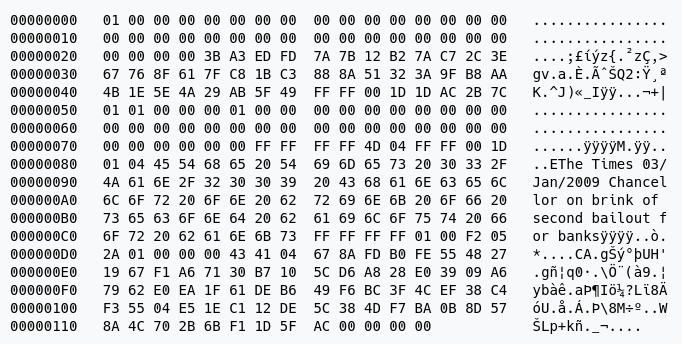
\includegraphics[width=90mm,scale=1.0]{./figs/genesis.png}
   \caption[Bloco g\^enesis da rede Bitcoin]{Conte\'udo do primeiro bloco - g\^enesis - da rede Bitcoin, com refer\^encia \`a manchete do dia 03 de Janeiro de 2009 do jornal ingl\^es The Times: "Tesouro brit\^anico \`a beira do segundo resgate para os bancos". Os governos inflacionaram suas moedas via artif\'icios como Quantitative Easing para cobrir a d\'ivida dos bancos insolventes.}
   \label{fig:genesis}
 \end{center}
\end{figure}

Por\'{e}m, por se tratar de uma inven\c{c}\~{a}o recente, sua exist\^{e}ncia ainda encontra-se longe do radar da maioria dos usu\'{a}rios conectados em rede.
De forma an\'{a}loga, a pr\'{o}pria Internet representou uma verdadeira mudan\c{c}a de paradigmas quando foi finalmente expandida para al\'{e}m das comunidades acad\^{e}micas e outros nichos mais espec\'{i}ficos, atingindo a popula\c{c}\~{a}o geral a partir da segunda metade da d\'{e}cada de 1990.
Por\'{e}m, cabe ressaltar que a mesma precisou ficar, de certa forma, incubada por muitos anos at\'{e} que alcan\c{c}asse o estado de maturidade necess\'{a}rio para ser adotada em massa\footnote{E.g. n\~ao \'e mais necess\'ario conhecimento t\'ecnico de protocolos como TCP/IP ou VoIP para utiliz\'a-los.}.

A aplicabilidade das \textit{blockchains} \'{e} diversa indo al\'{e}m de somente suportar o funcionamento de moeda de troca e apenas os anos que seguir\~{a}o v\~{a}o poder confirmar sua verdadeira utilidade.
Acredita-se que cada vez mais casos de uso ser\~{a}o implementados neste novo paradigma descentralizado por conta do argumento de incentivo econ\^{o}mico.
%Para corroborar, um \textit{survey} com motoristas da Uber para que analisassem a possibilidade de mudan\c{c}a para um aplicativo concorrente descentralizado hipot\'{e}tico que n\~{a}o cobrasse 25\% de taxa em suas receitas poderia ser proposto.
Ao possibilitar que os membros de uma comunidade que tanto criam quanto extraem valor da mesma criem um la\c{c}o econ\^{o}mico eficiente entre si sem a necessidade de intermedi\'{a}rios, tornam-se mais pr\'{o}ximos da figura cl\'{a}ssica de um \textit{stakeholder} e t\^{e}m seus interesses alinhados.
Assim, novas formas de organiza\c{c}\~{o}es sociais e econ\^{o}micas surgir\~{a}o.

Entretanto, muitos desafios ainda se encontram com solu\c{c}\~{a}o em aberto para a maioria das \textit{blockchains}.
Especificamente no \^{a}mbito do protocolo Bitcoin, muitos fatores devem ser levados em considera\c{c}\~{a}o na tentativa de realizar uma proje\c{c}\~{a}o de seu sucesso futuro.
Seu algoritmo de for\c{c}a bruta, tamb\'{e}m adotado ainda na maioria das outras \textit{blockchains}, \'{e} respons\'{a}vel por incentivar o consumo desenfreado de energia el\'{e}trica pelos n\'{o}s mineiros, o que pode acabar por torn\'{a}-lo ecologicamente insustent\'{a}vel no longo prazo.
Seu modelo de cobrar taxas em cada transa\c{c}\~{a}o, apesar de pr\'{a}tica comum em todos os sistemas de pagamento mais utilizados at\'{e} ent\~{a}o, \'e criticado desde por quest\~oes financeiras at\'e pela simples experi\^encia de usu\'ario.
Potenciais problemas como a quebra das fun\c{c}\~{o}es criptogr\'{a}ficas utilizadas com o advento da computa\c{c}\~{a}o qu\^{a}ntica n\~{a}o podem ser ignorados numa an\'{a}lise mais ampla.
Entretanto, a falta de um plano concreto para escalar a \textit{blockchain} para quantos usu\'{a}rios necess\'{a}rios, a inexist\^{e}ncia de governan\c{c}a para ditar as regras de implementa\c{c}\~{a}o de inova\c{c}\~{o}es exigidas pela comunidade e a centraliza\c{c}\~{a}o do \textit{hashrate} em pouqu\'{i}ssimas empresas mineradoras s\~{a}o os problemas mais pertinentes.

\singlespacing
\bibliographystyle{abntex2-alf}
\bibliography{referencias}

\end{document}
